\section{Strain Analysis and Discussion}
 
\graphicspath{{Chapter4/Figs/}}

\begin{frame}
 \frametitle{Strain Analysis}
 \framesubtitle{}
 \label{ch4:}
 
  Model parameters for Shen algorithm
  
  Data Set: MIDAS
  \begin{itemize}
    \item Wt=6
    \item dmin = 1km
    \item dmax = 500km
    \item dstep = 1km
    \item ltype = gaussian
    \item x step = y step = 0.5 $^{\circ}$
    \item region = Greece: 18/30/34/43 -  Italy: 4/18/32/48
  \end{itemize}

\end{frame}
\note{}

\begin{frame}
 \frametitle{Strain Analysis}
 \framesubtitle{Greece region}
 \label{ch4:}
   
  \begin{columns}
    \begin{column}{0.5\textwidth}
      
      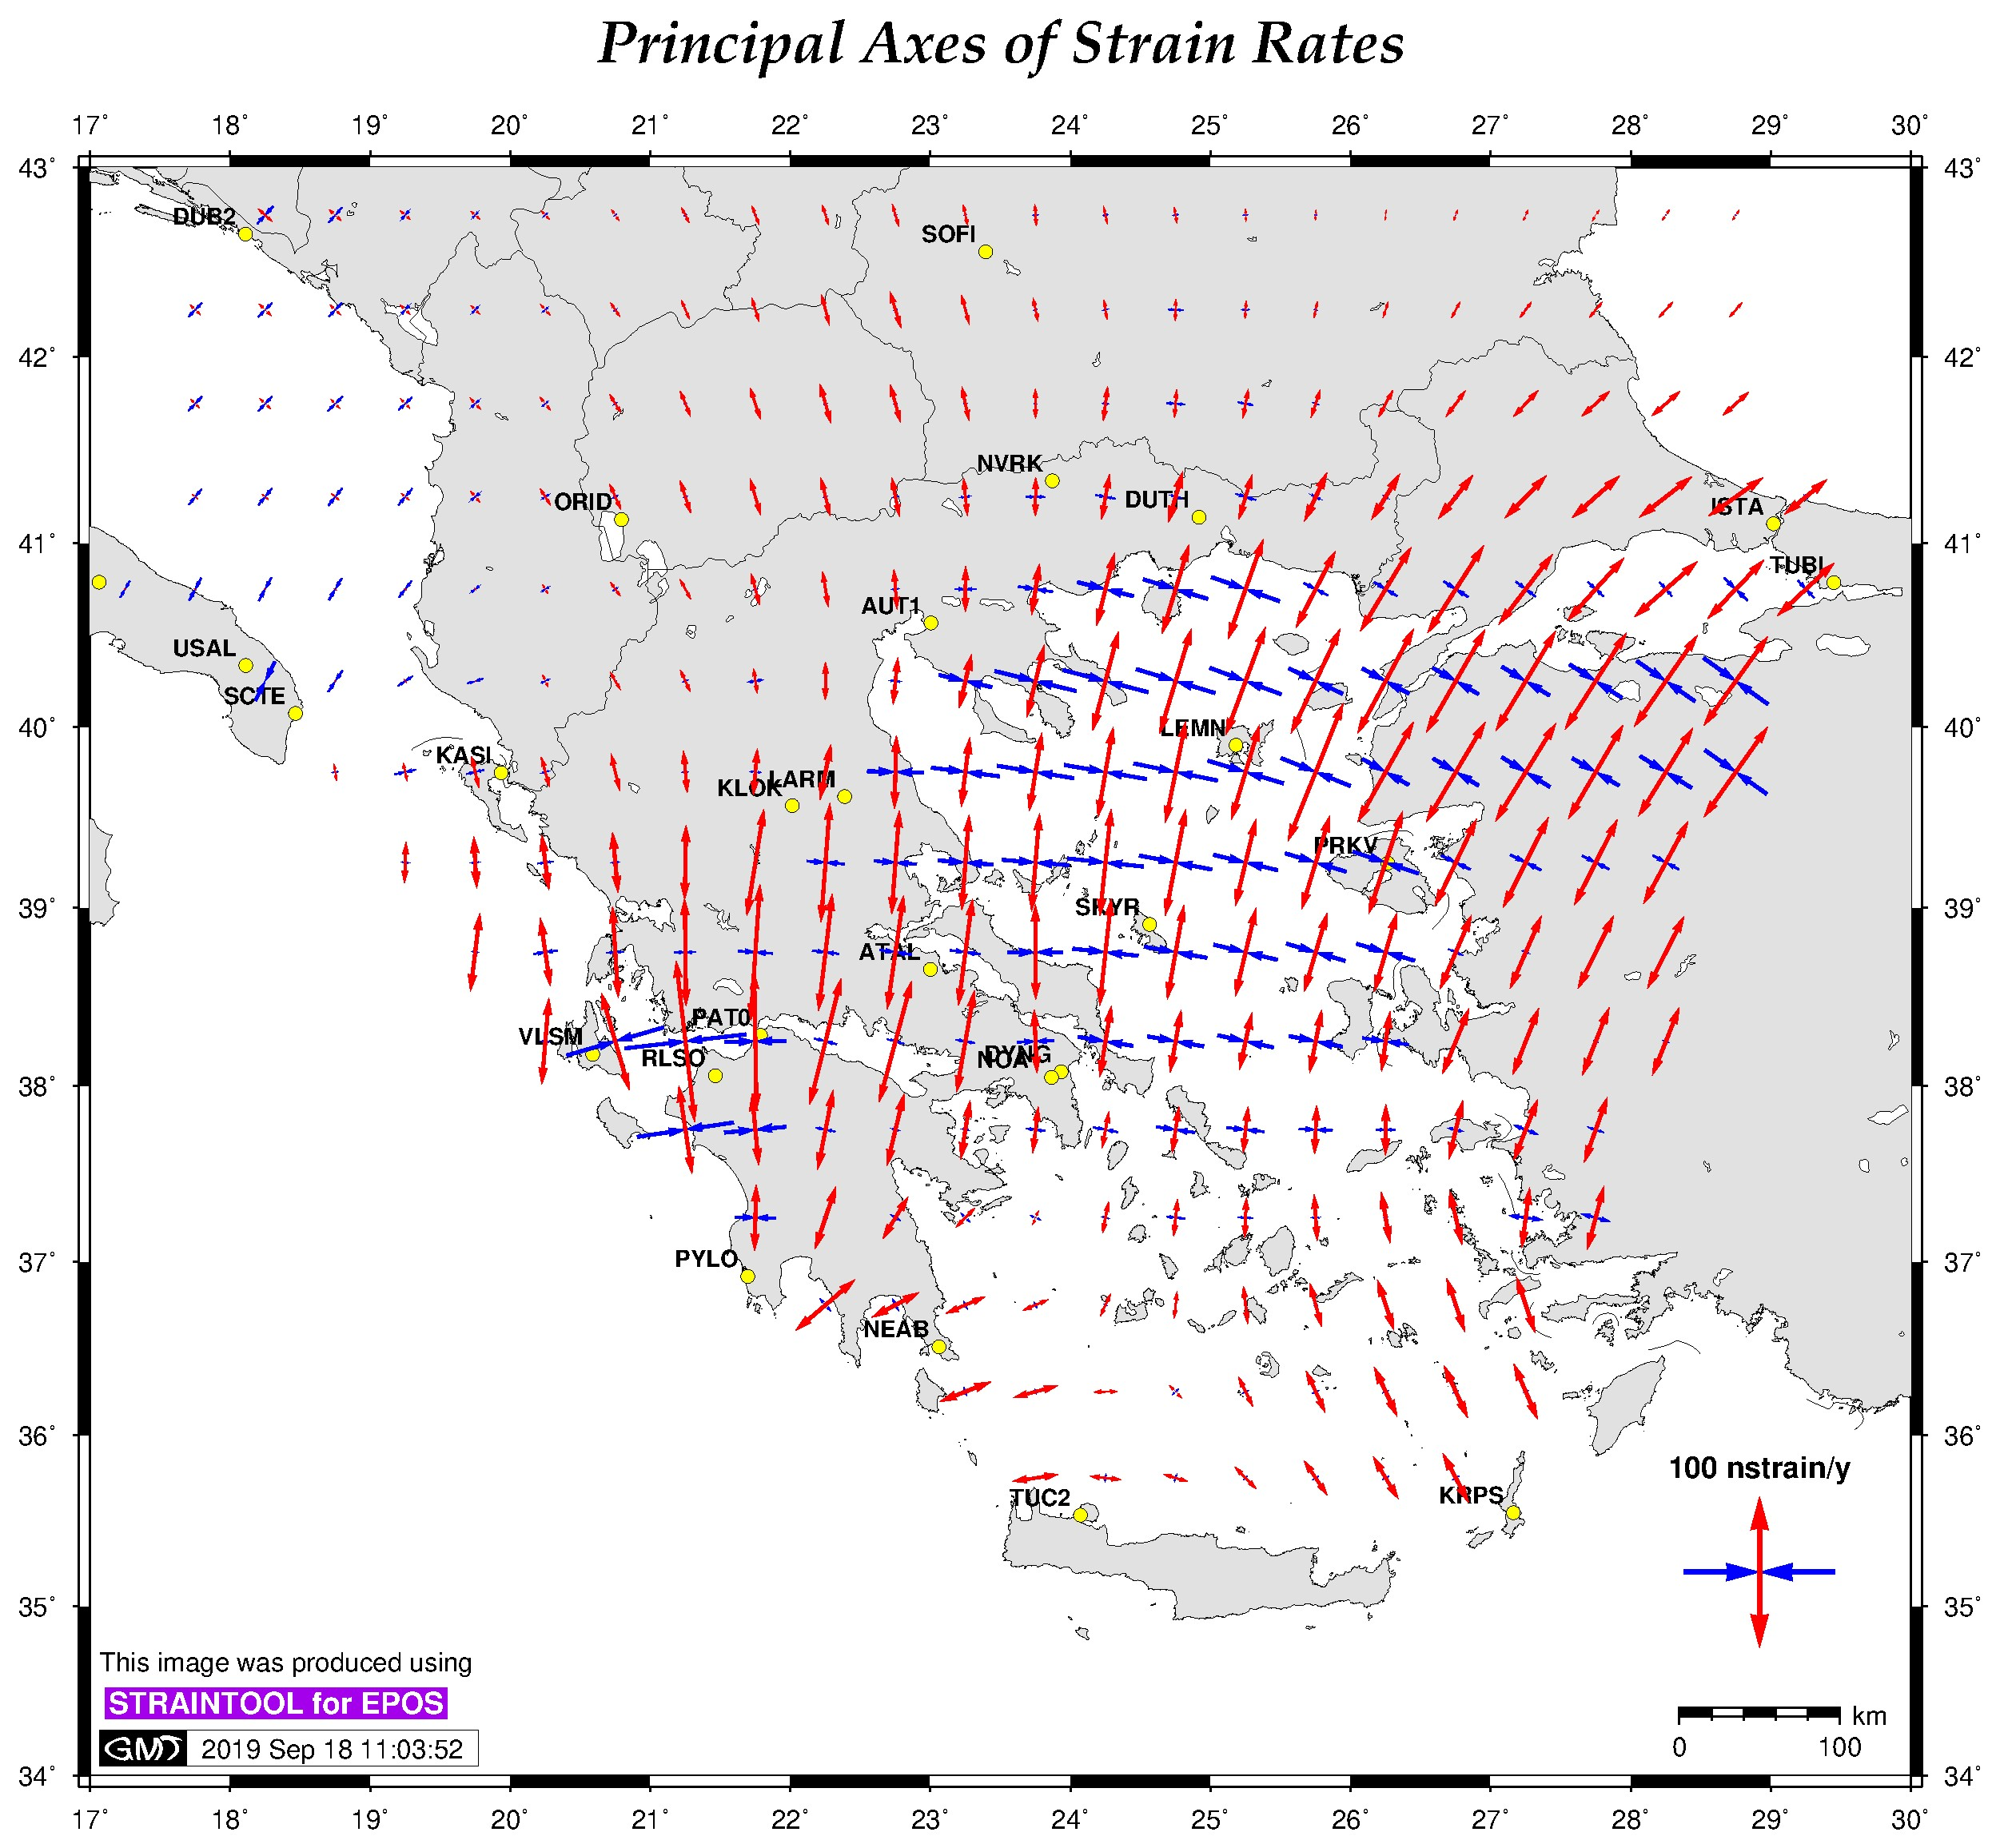
\includegraphics[width=.9\textwidth]{grmidas-output_str.jpg}   
    \end{column}
    \begin{column}{0.5\textwidth}
    \begin{center}
      
      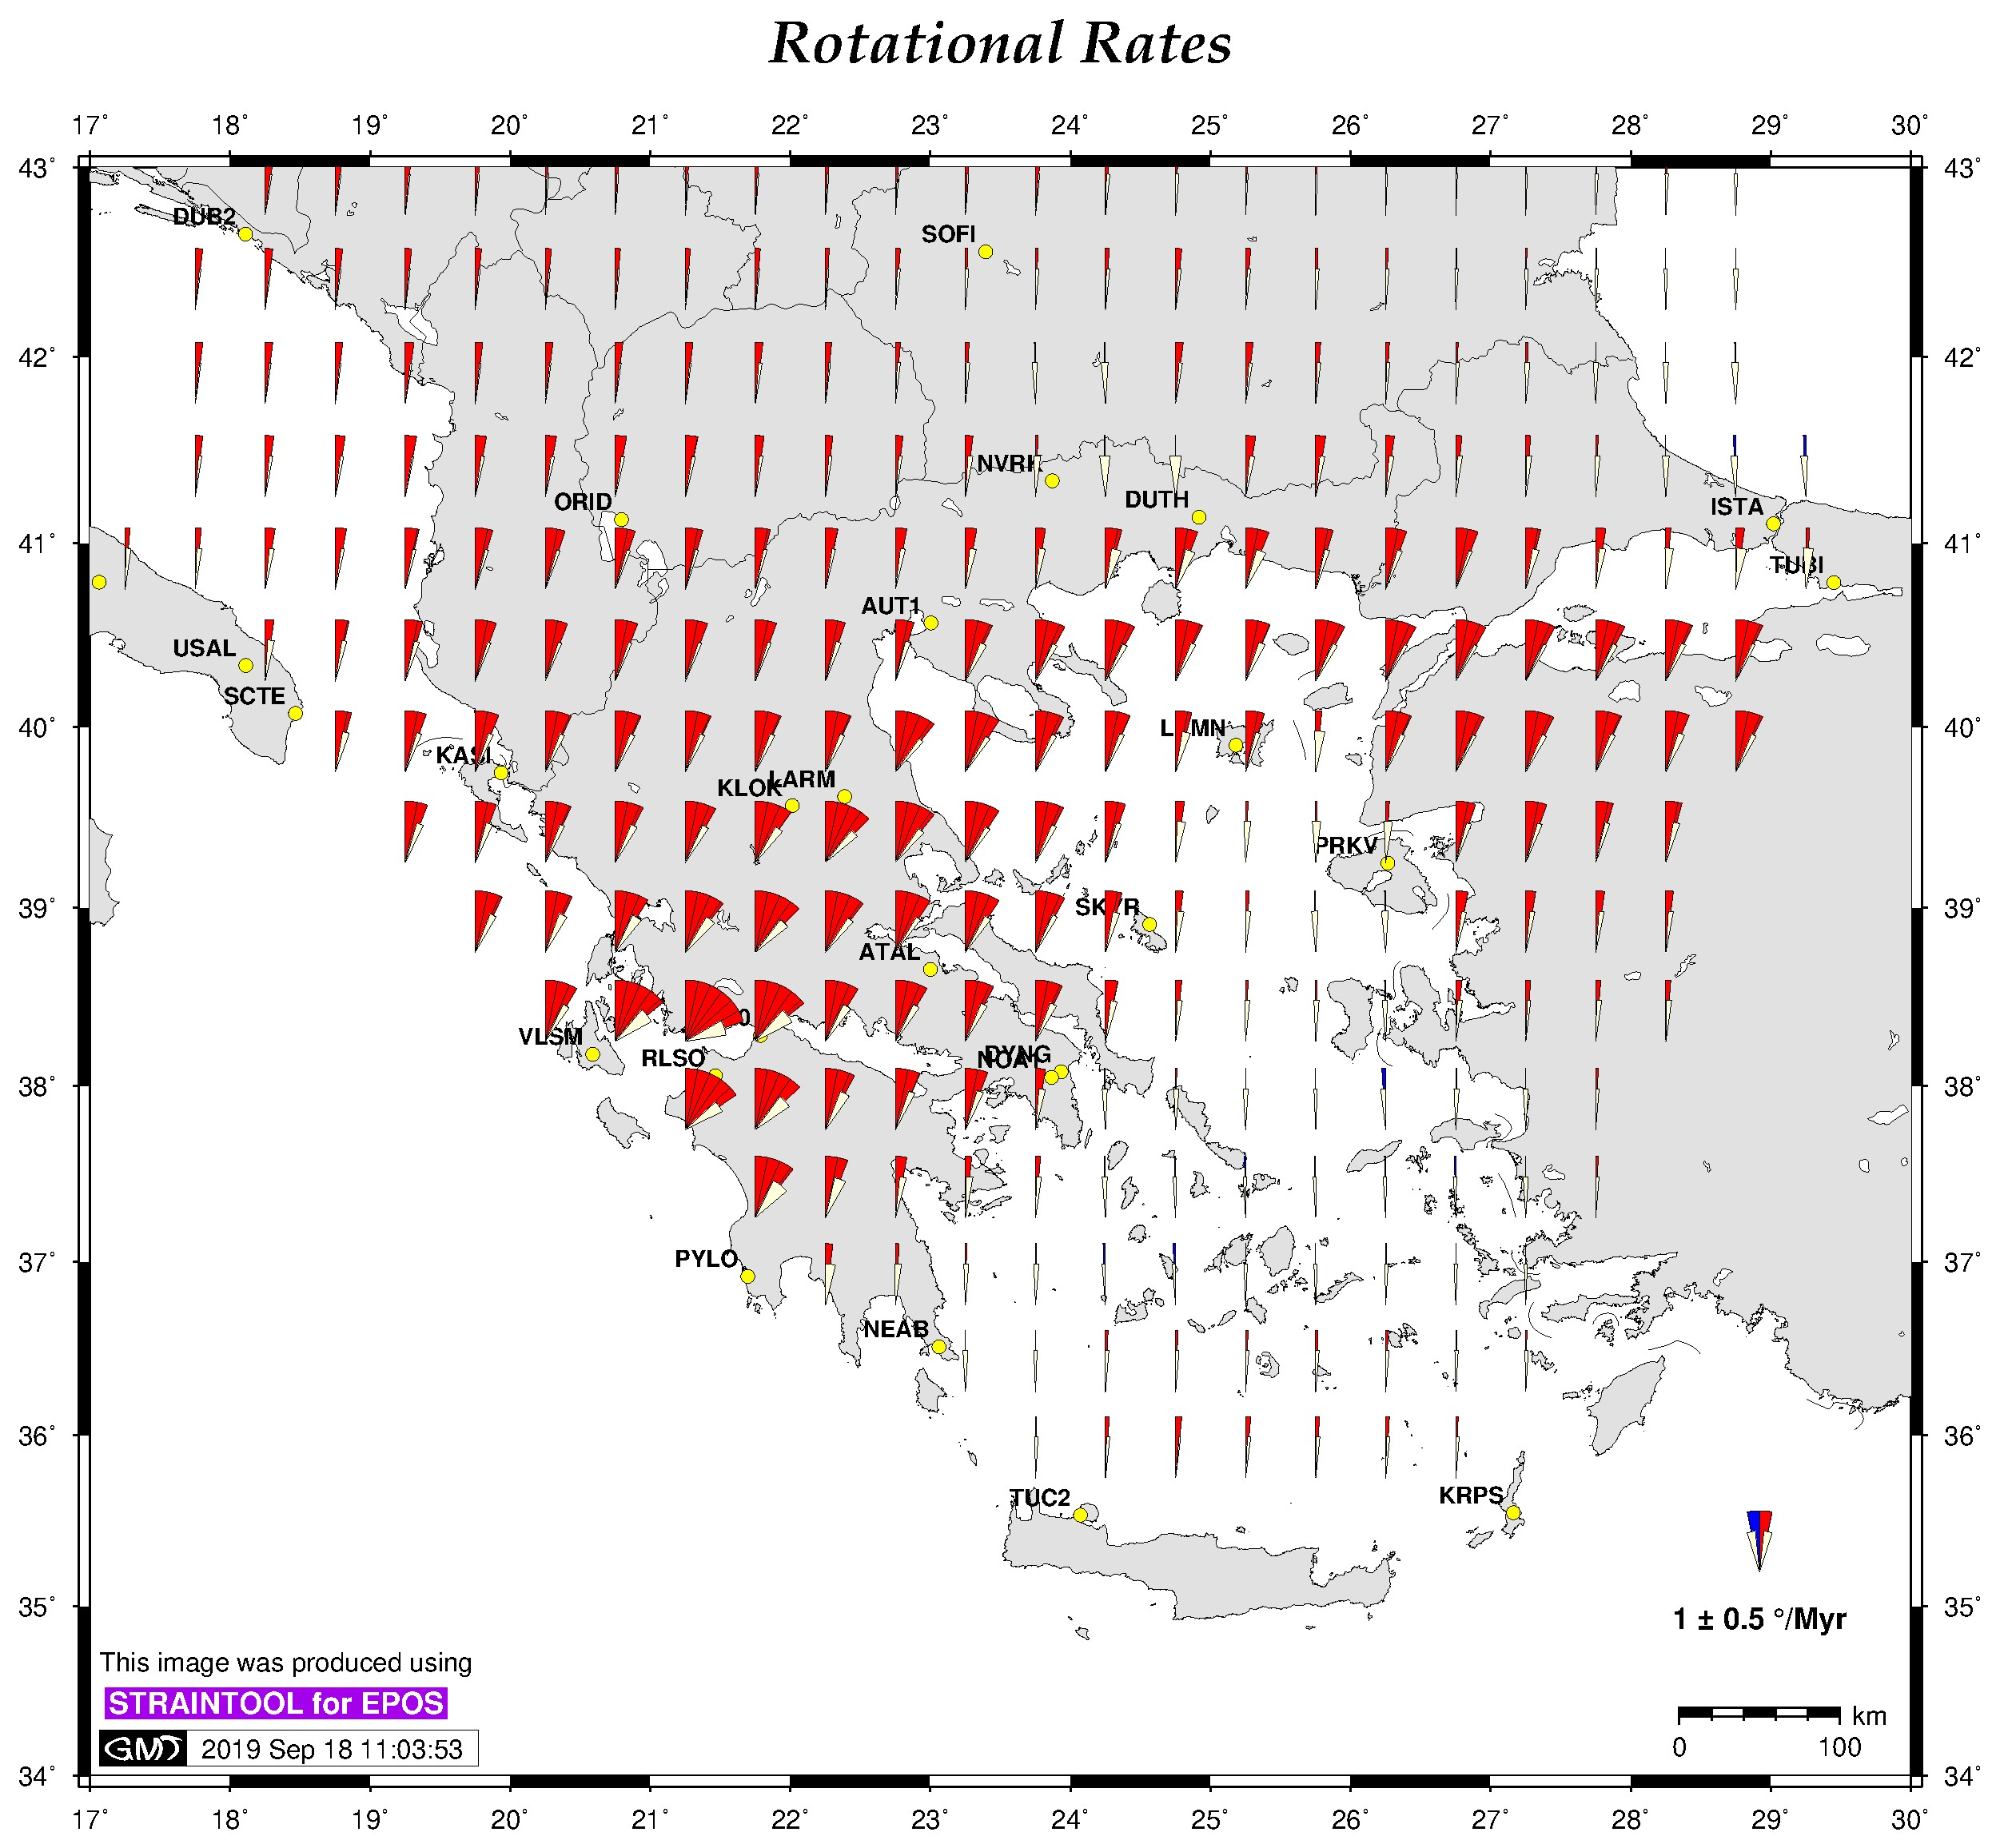
\includegraphics[width=0.9\textwidth]{grmidas-output_rot.jpg}     
    \end{center}
    \end{column}
  \end{columns}

\end{frame}
\note{}

\begin{frame}
 \frametitle{Strain Analysis}
 \framesubtitle{Greece region}
 \label{ch4:}
   
  \begin{columns}
    \begin{column}{0.5\textwidth}
      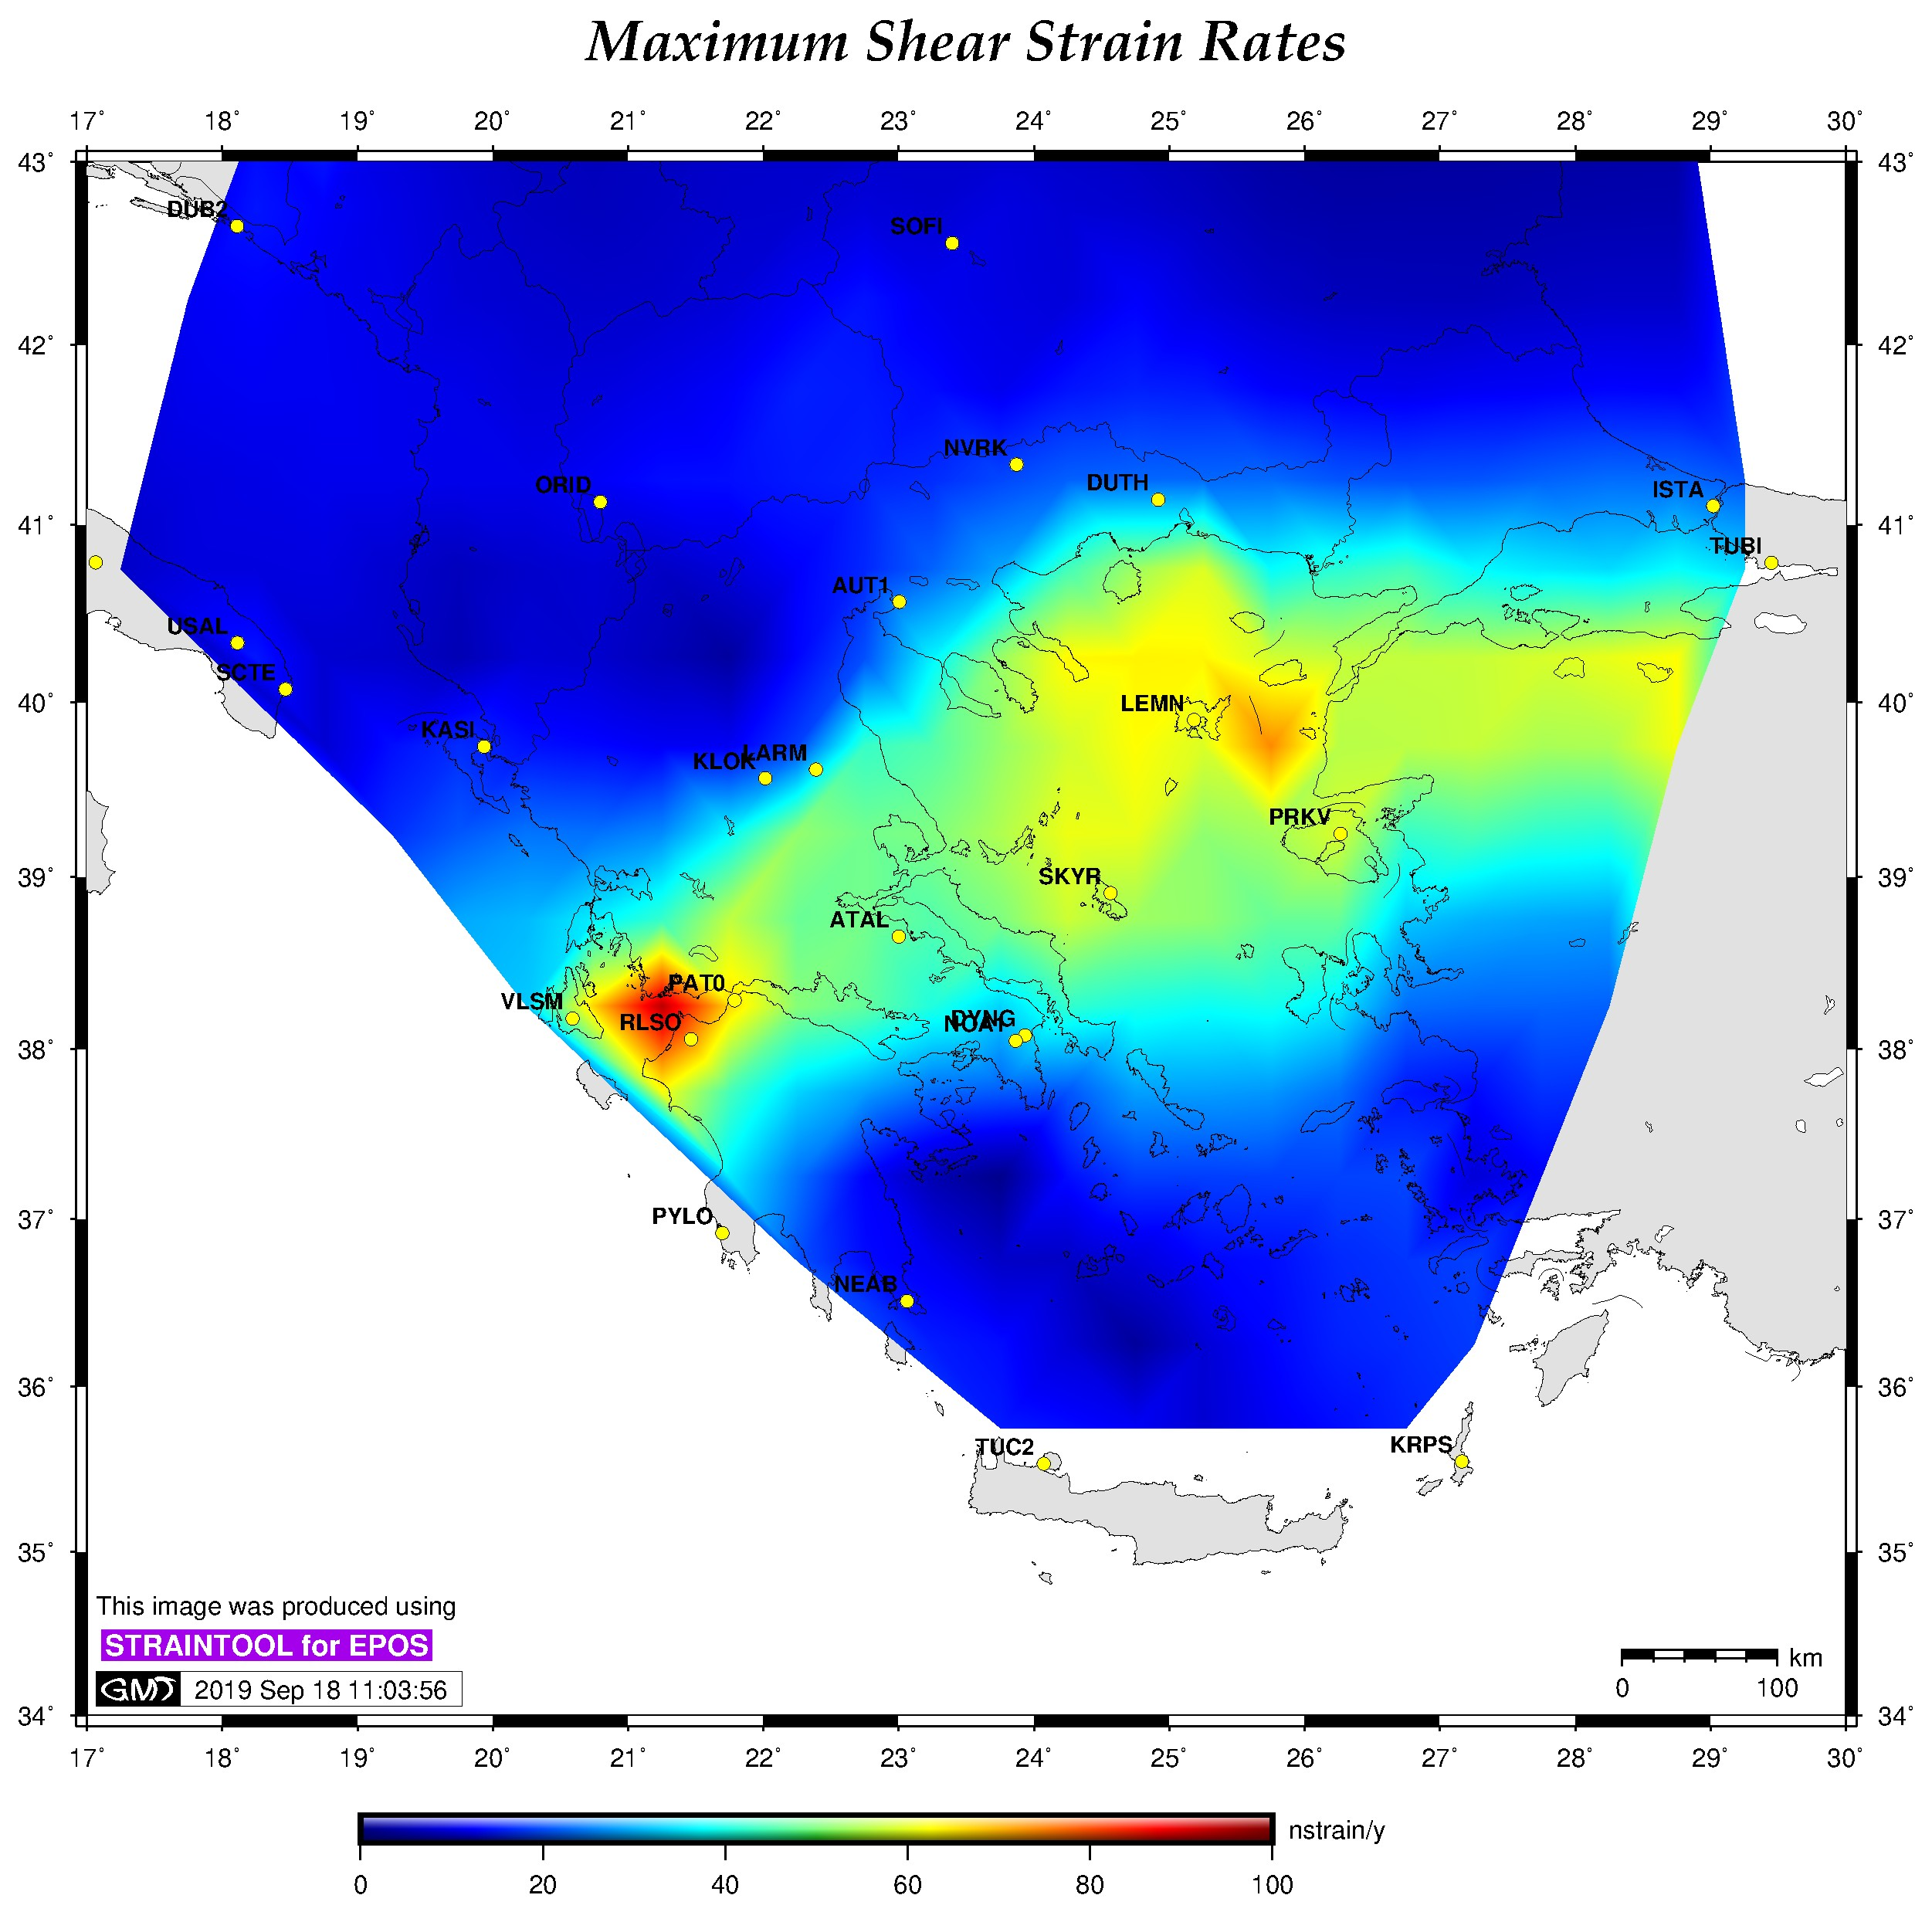
\includegraphics[width=.9\textwidth]{grmidas-output_gtot.jpg}   
    \end{column}
    \begin{column}{0.5\textwidth}
    \begin{center}
      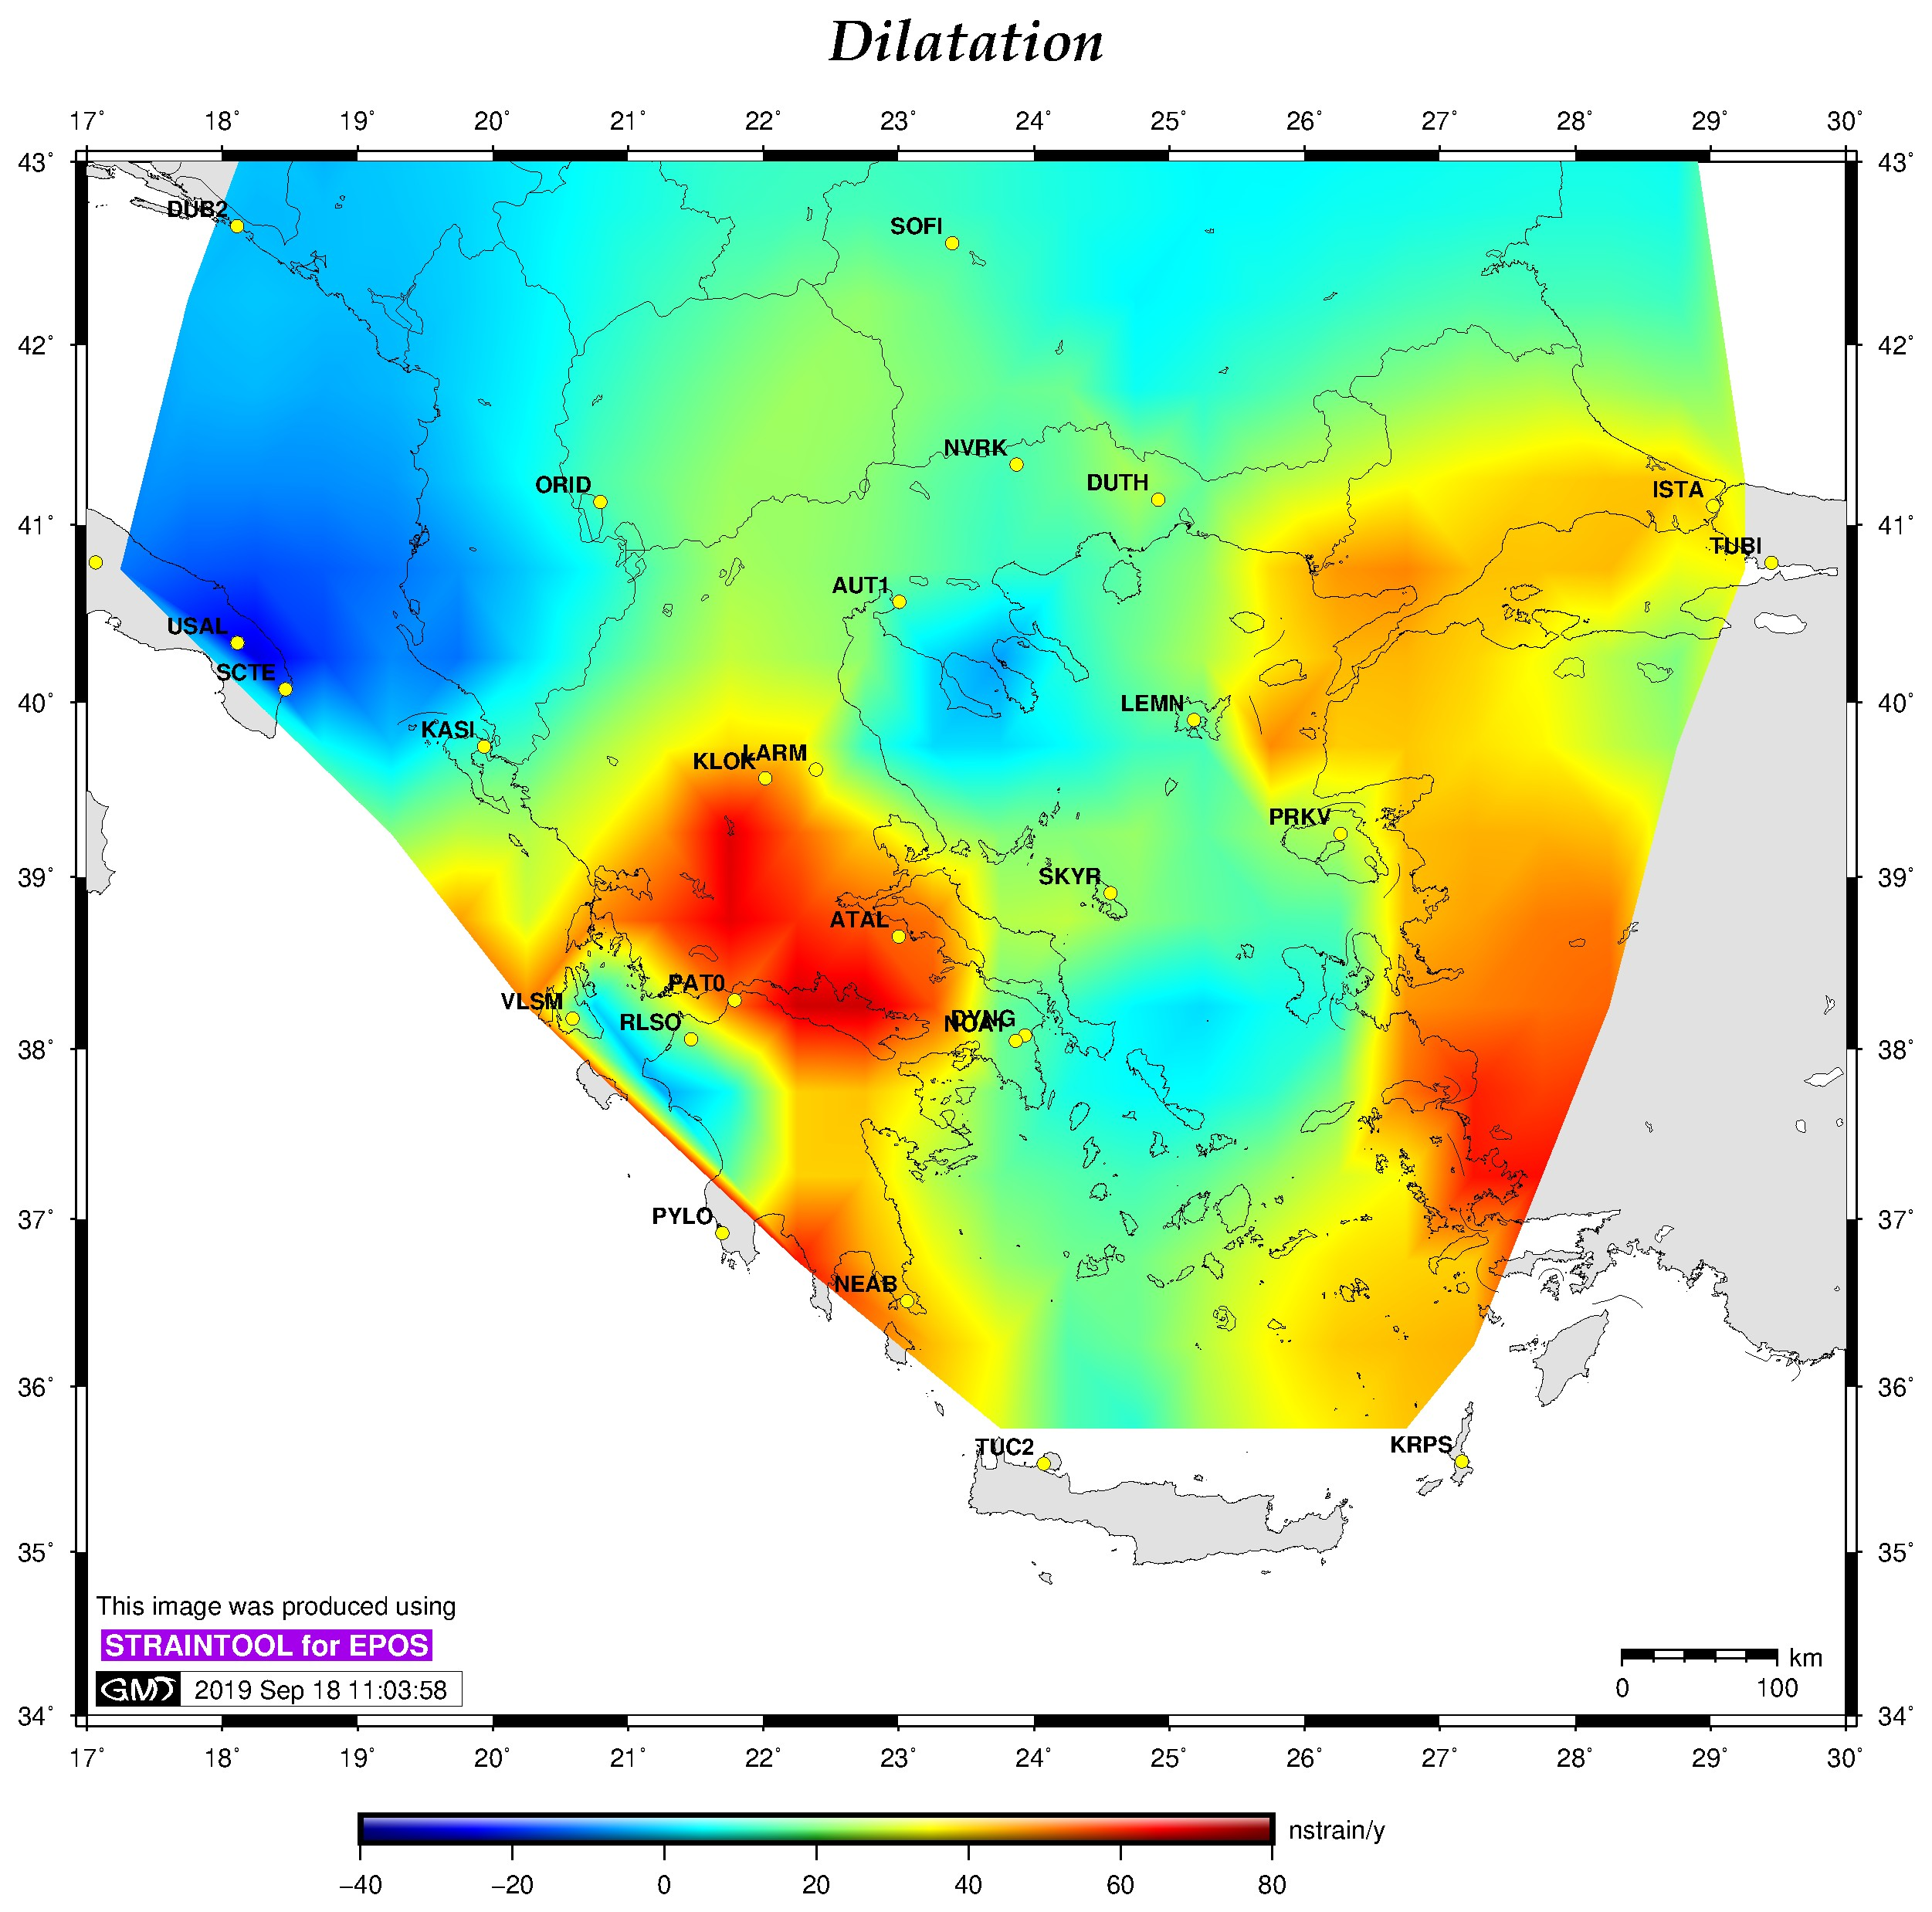
\includegraphics[width=0.9\textwidth]{grmidas-output_dil.jpg}     
    \end{center}
    \end{column}
  
  \end{columns}

\end{frame}
\note{}


\begin{frame}
 \frametitle{Strain Analysis}
 \framesubtitle{Greece region}
 \label{ch4:}
   
  \begin{columns}
    \begin{column}{0.5\textwidth}
      
      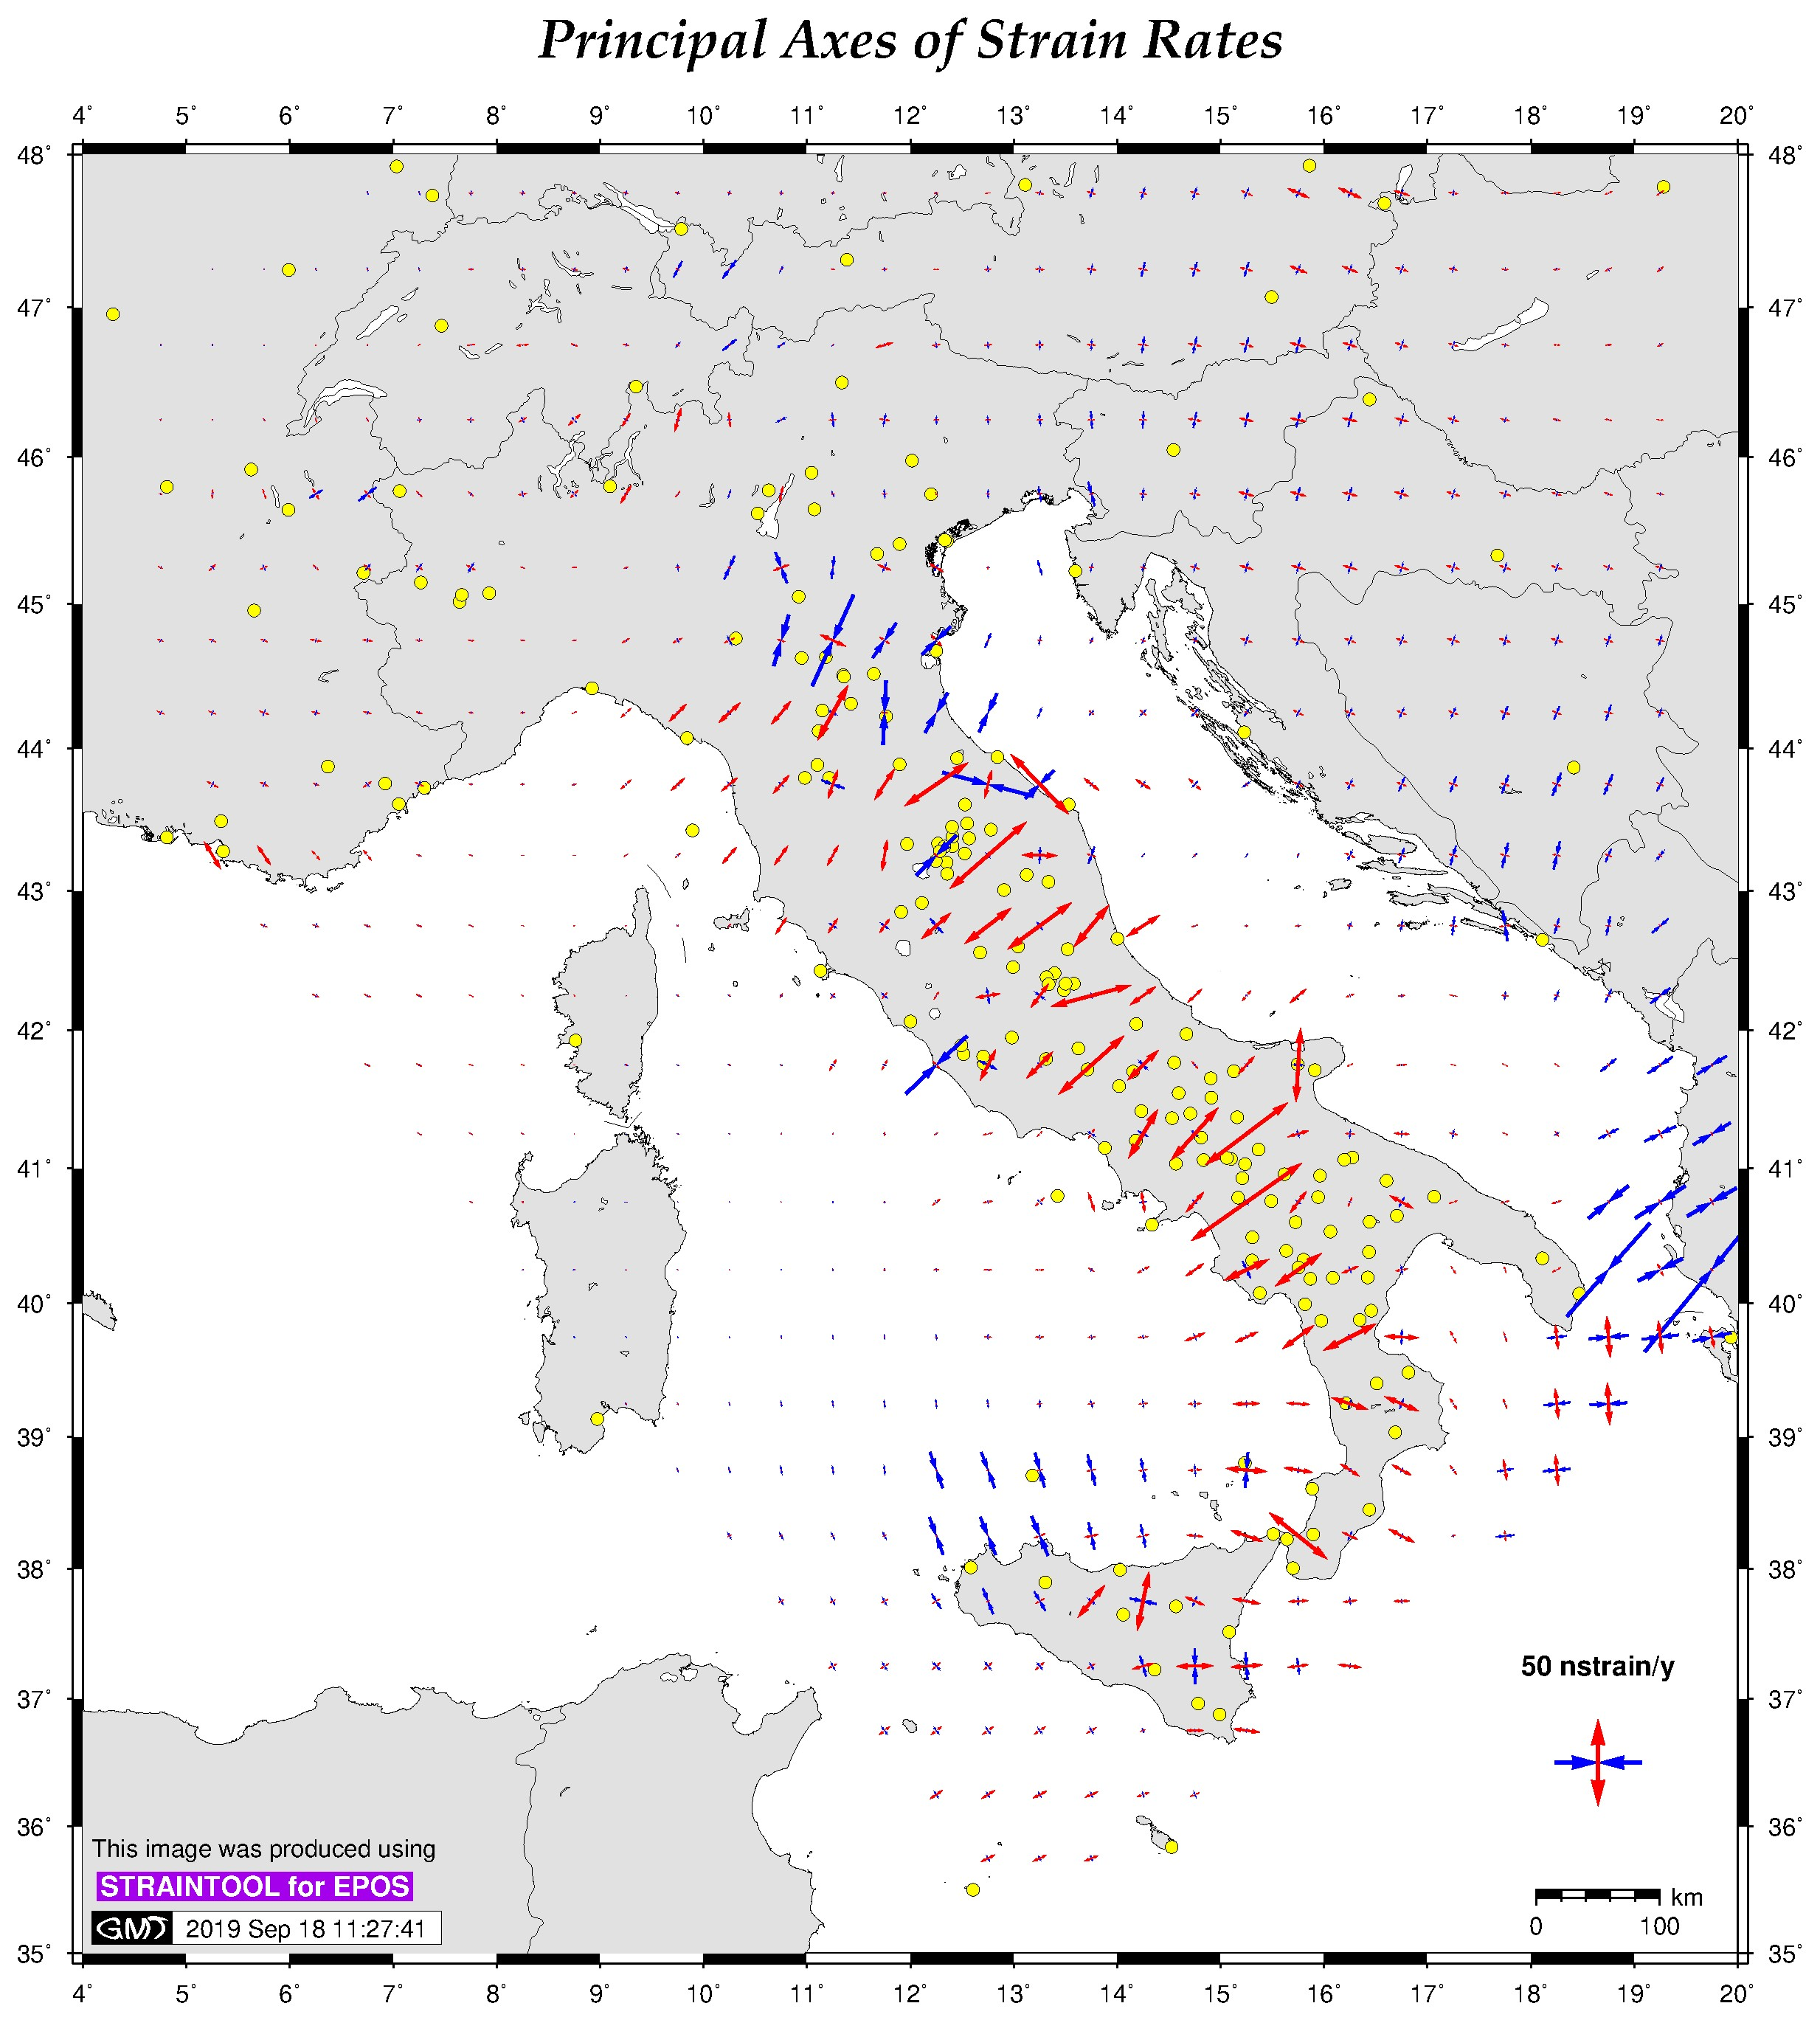
\includegraphics[width=.9\textwidth]{itmidas-output_str.jpg}   
    \end{column}
    \begin{column}{0.5\textwidth}
    \begin{center}
      
      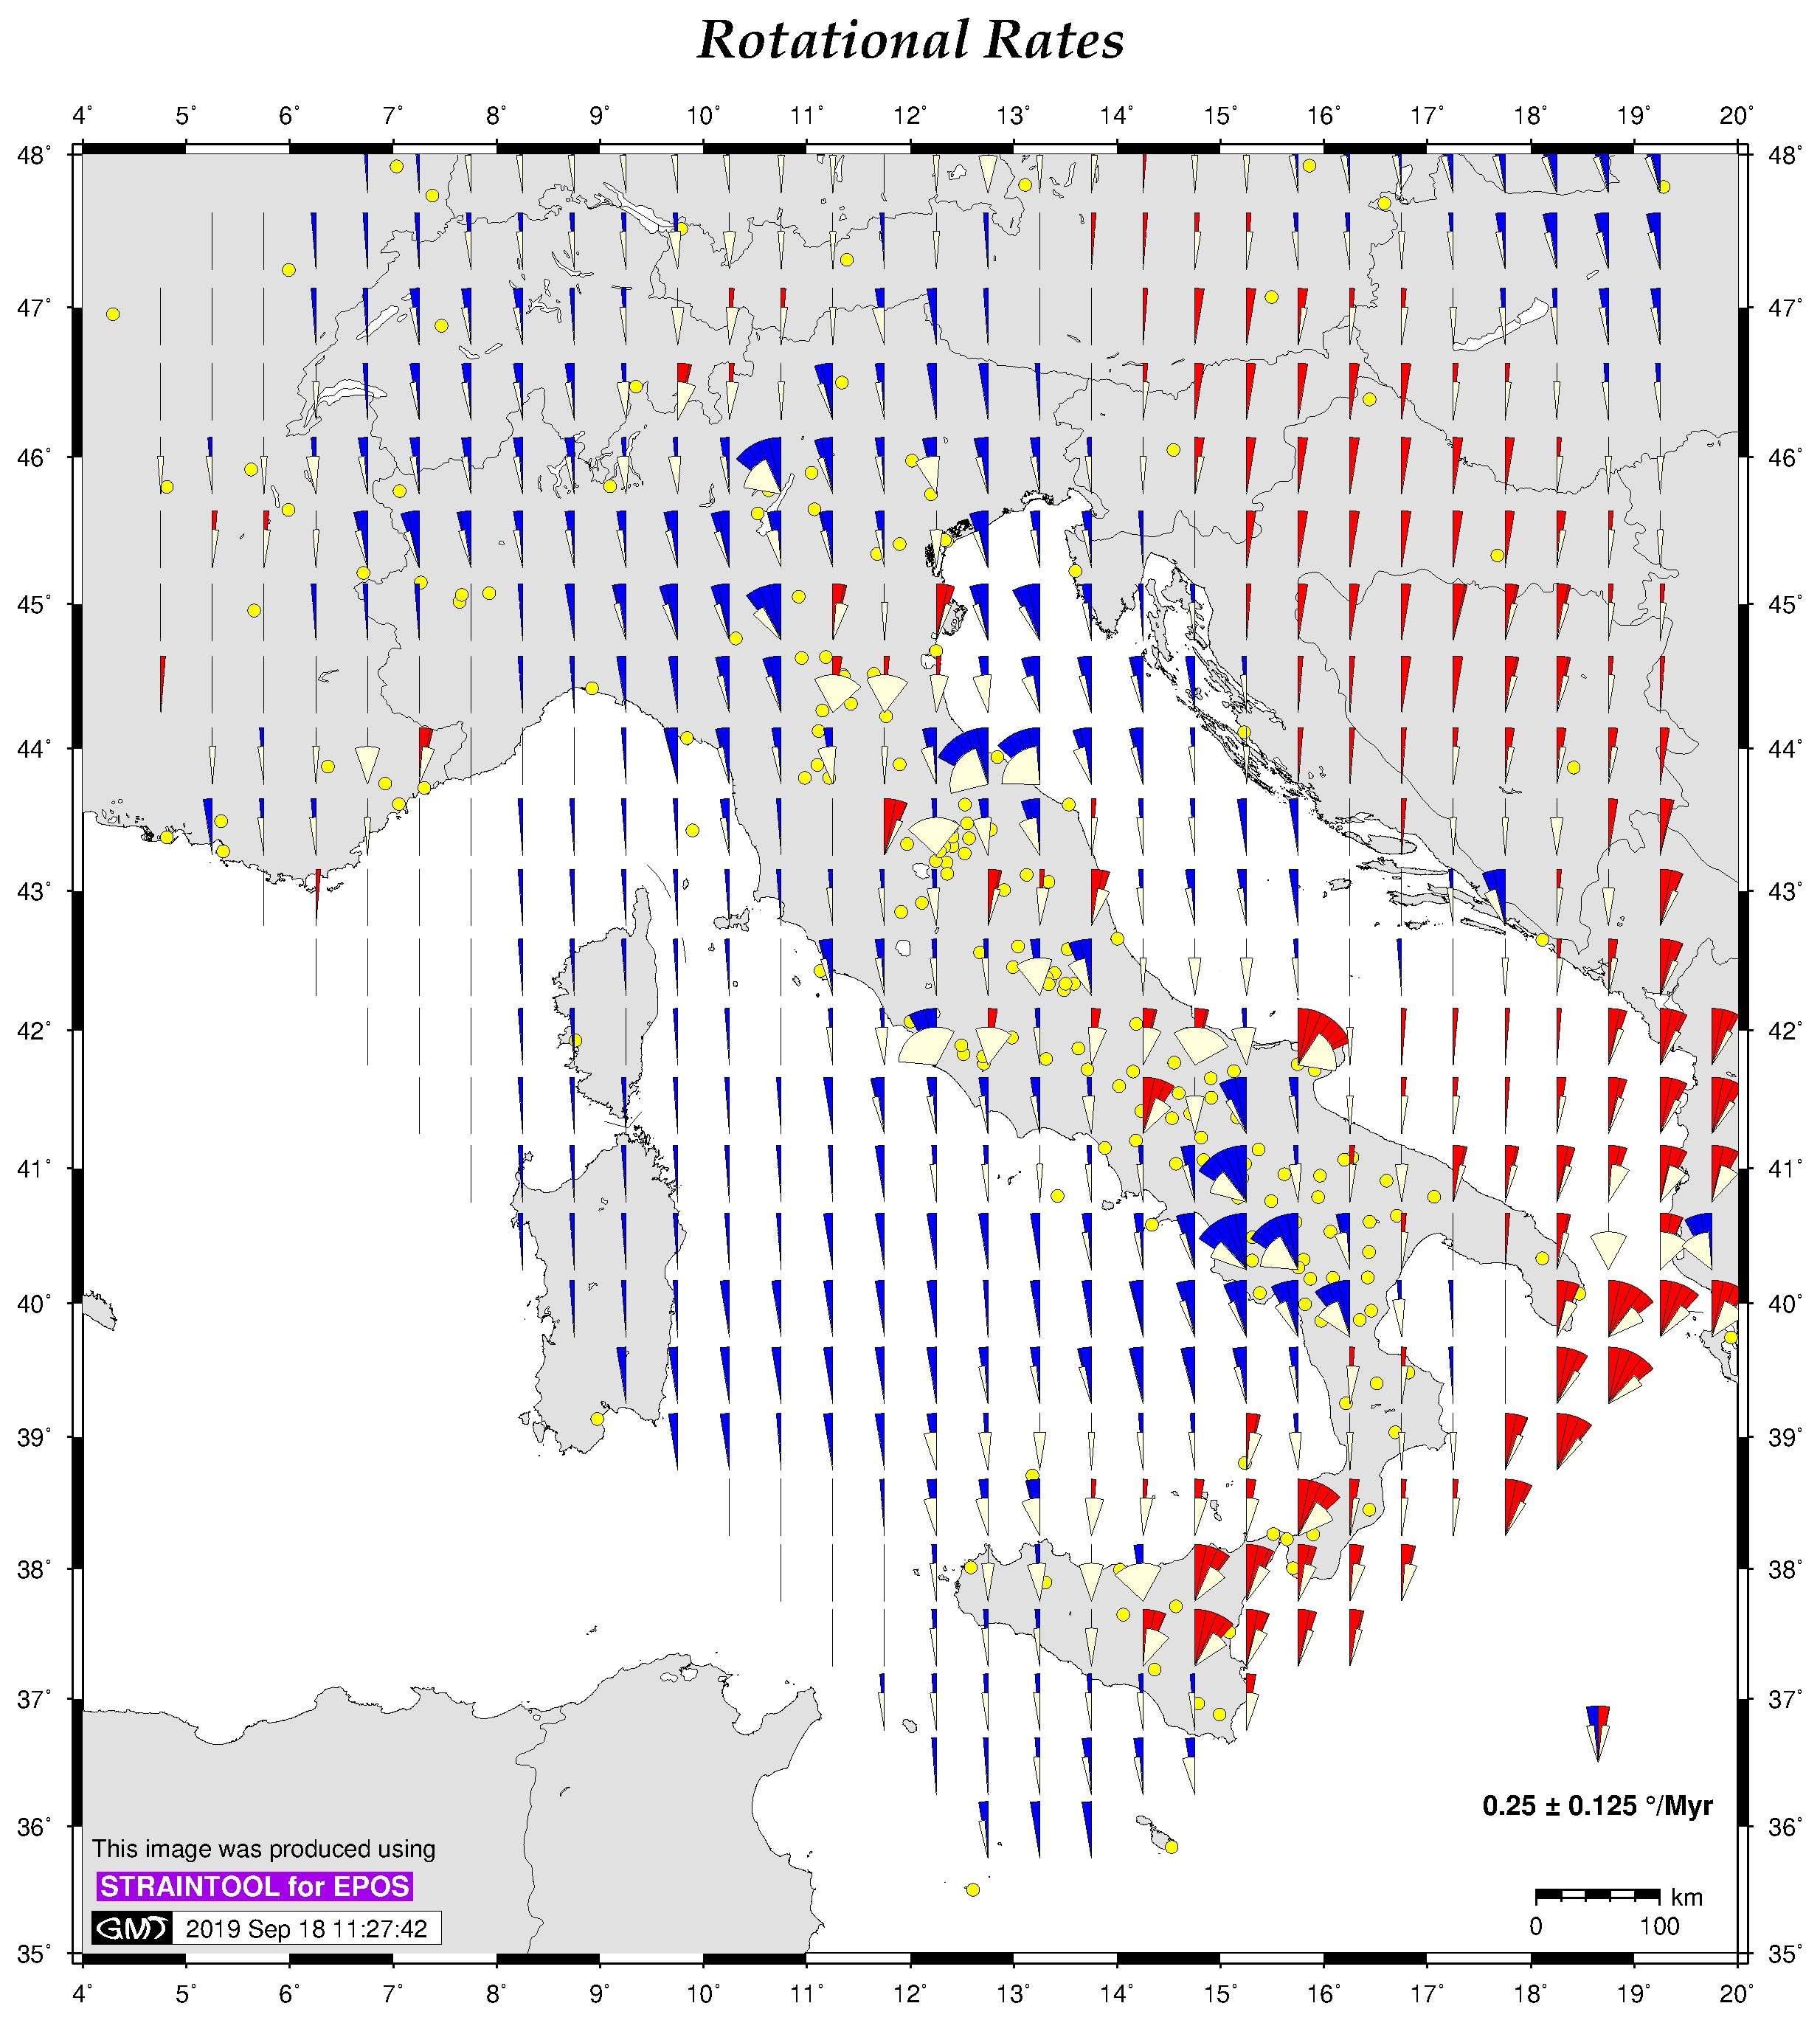
\includegraphics[width=0.9\textwidth]{itmidas-output_rot.jpg}     
    \end{center}
    \end{column}
  \end{columns}

\end{frame}
\note{}

\begin{frame}
 \frametitle{Strain Analysis}
 \framesubtitle{Greece region}
 \label{ch4:}
   
  \begin{columns}
    \begin{column}{0.5\textwidth}
      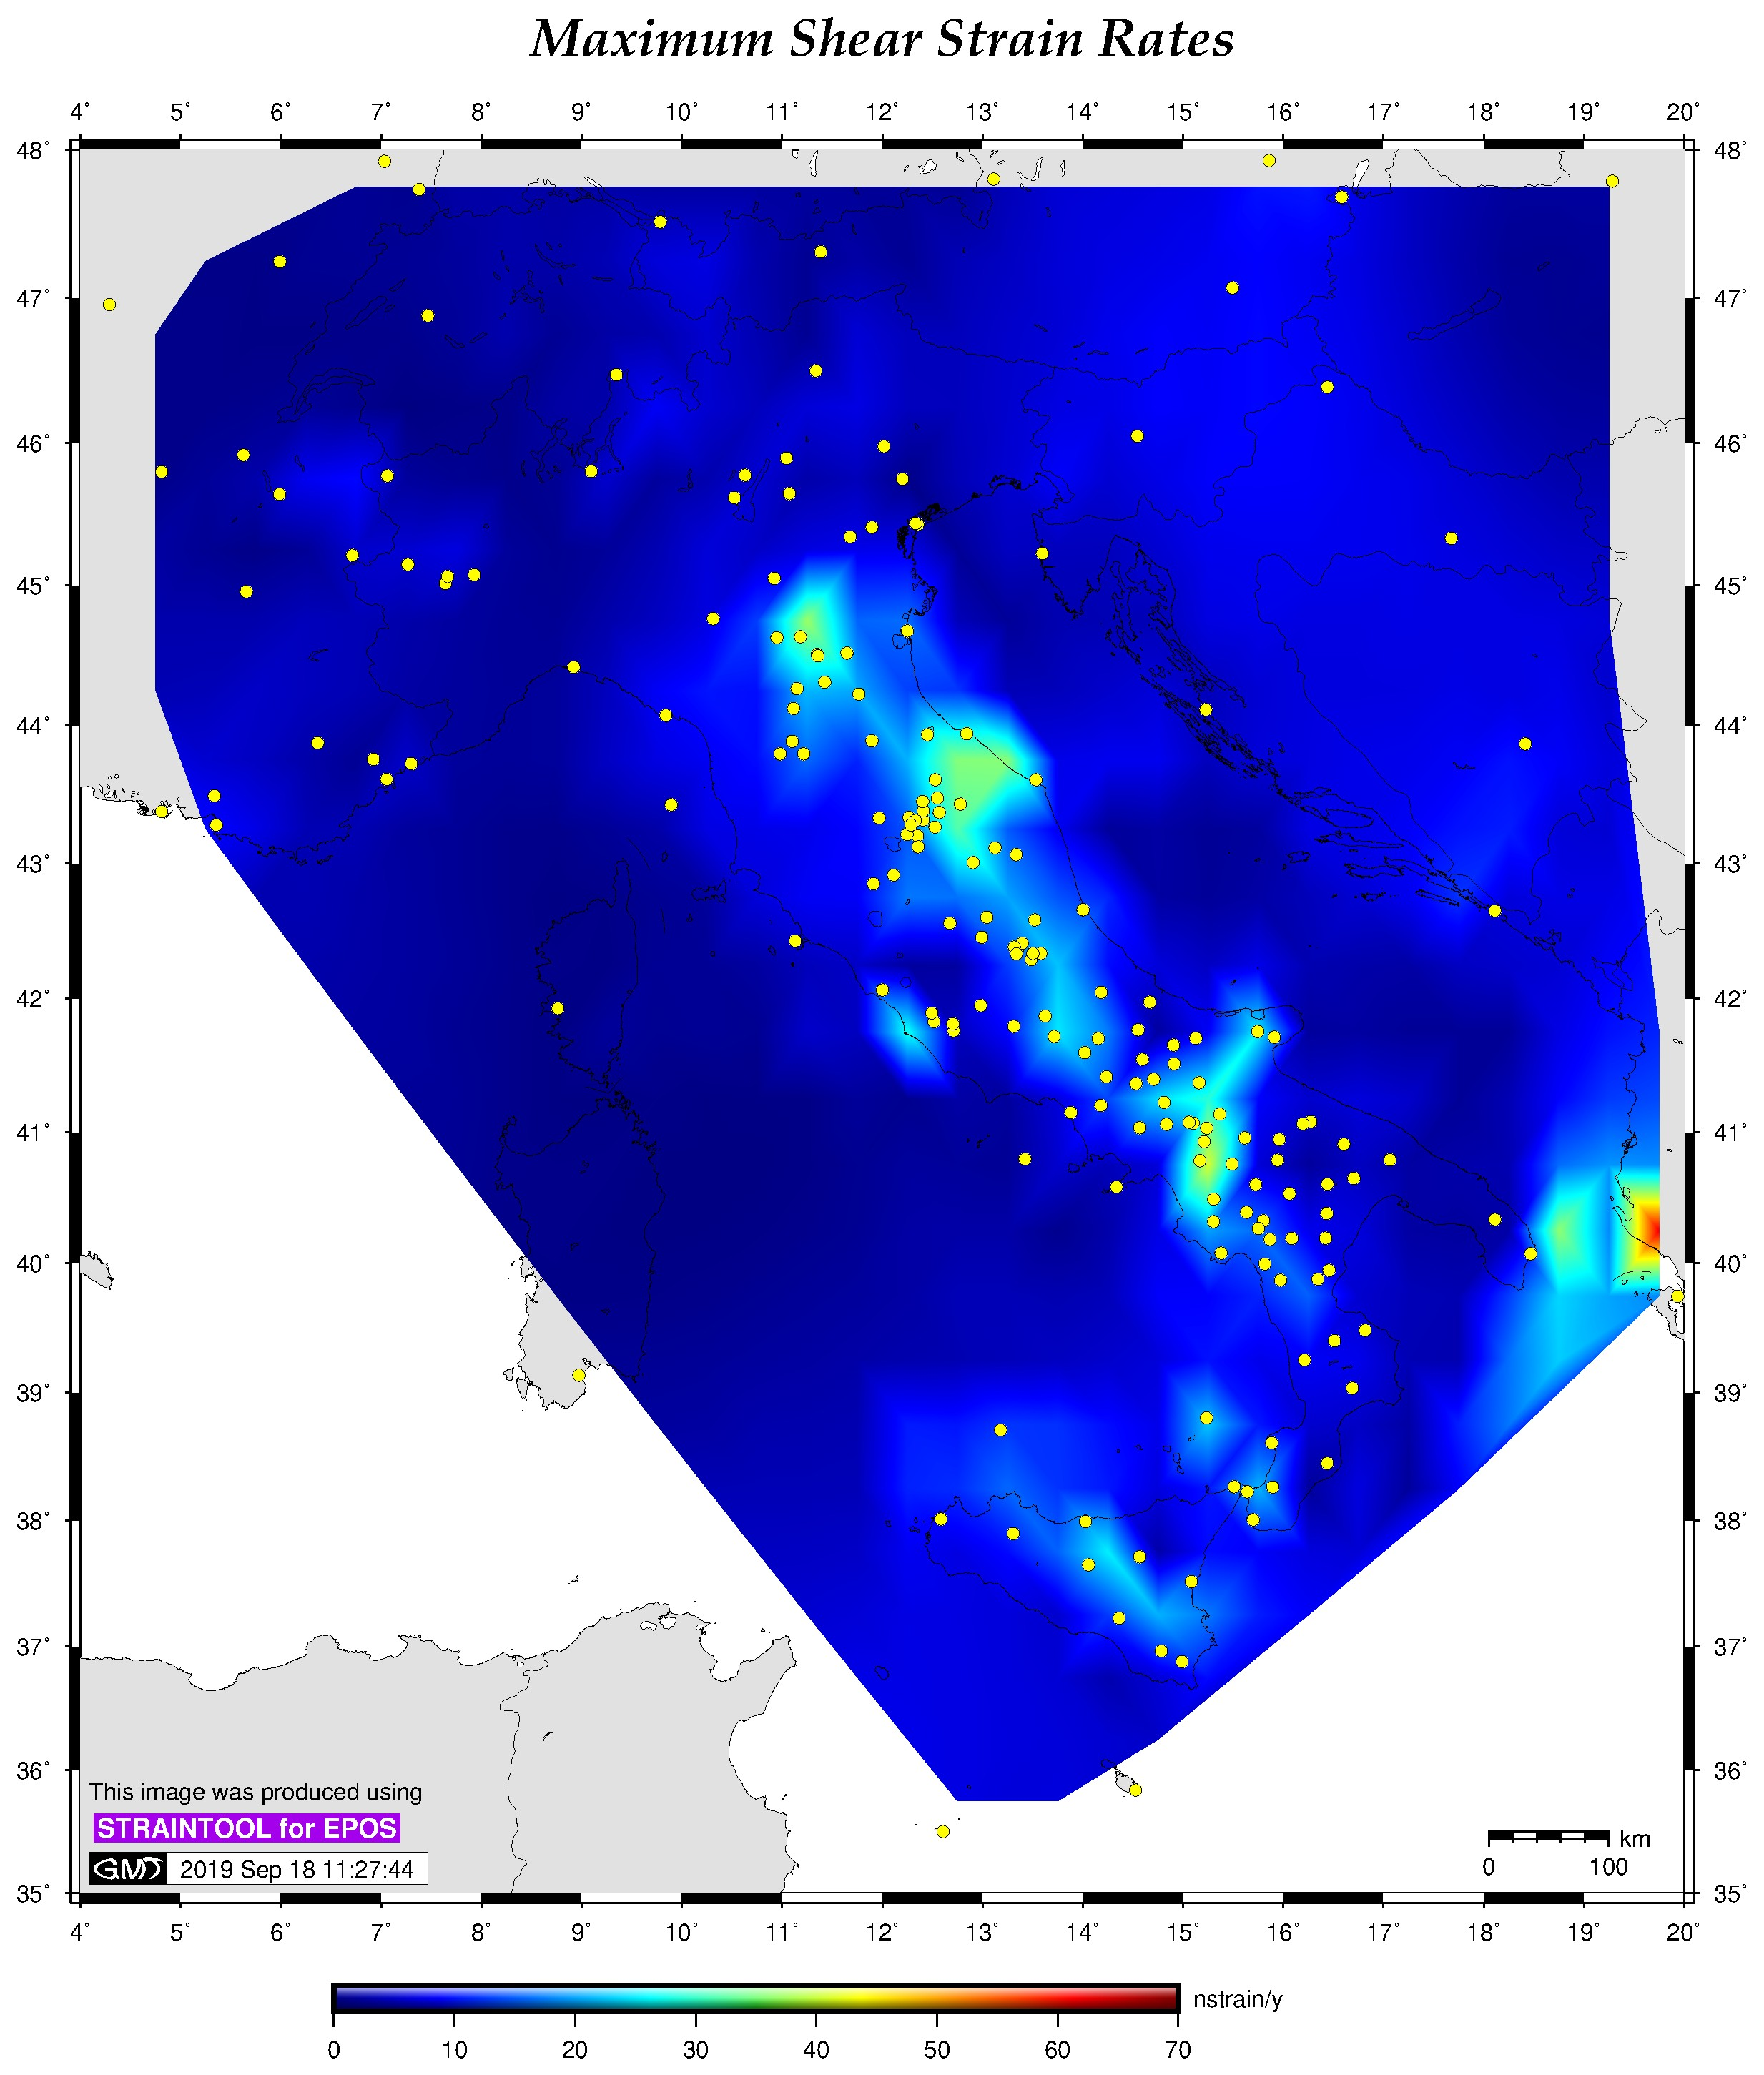
\includegraphics[width=.9\textwidth]{itmidas-output_gtot.jpg}   
    \end{column}
    \begin{column}{0.5\textwidth}
    \begin{center}
      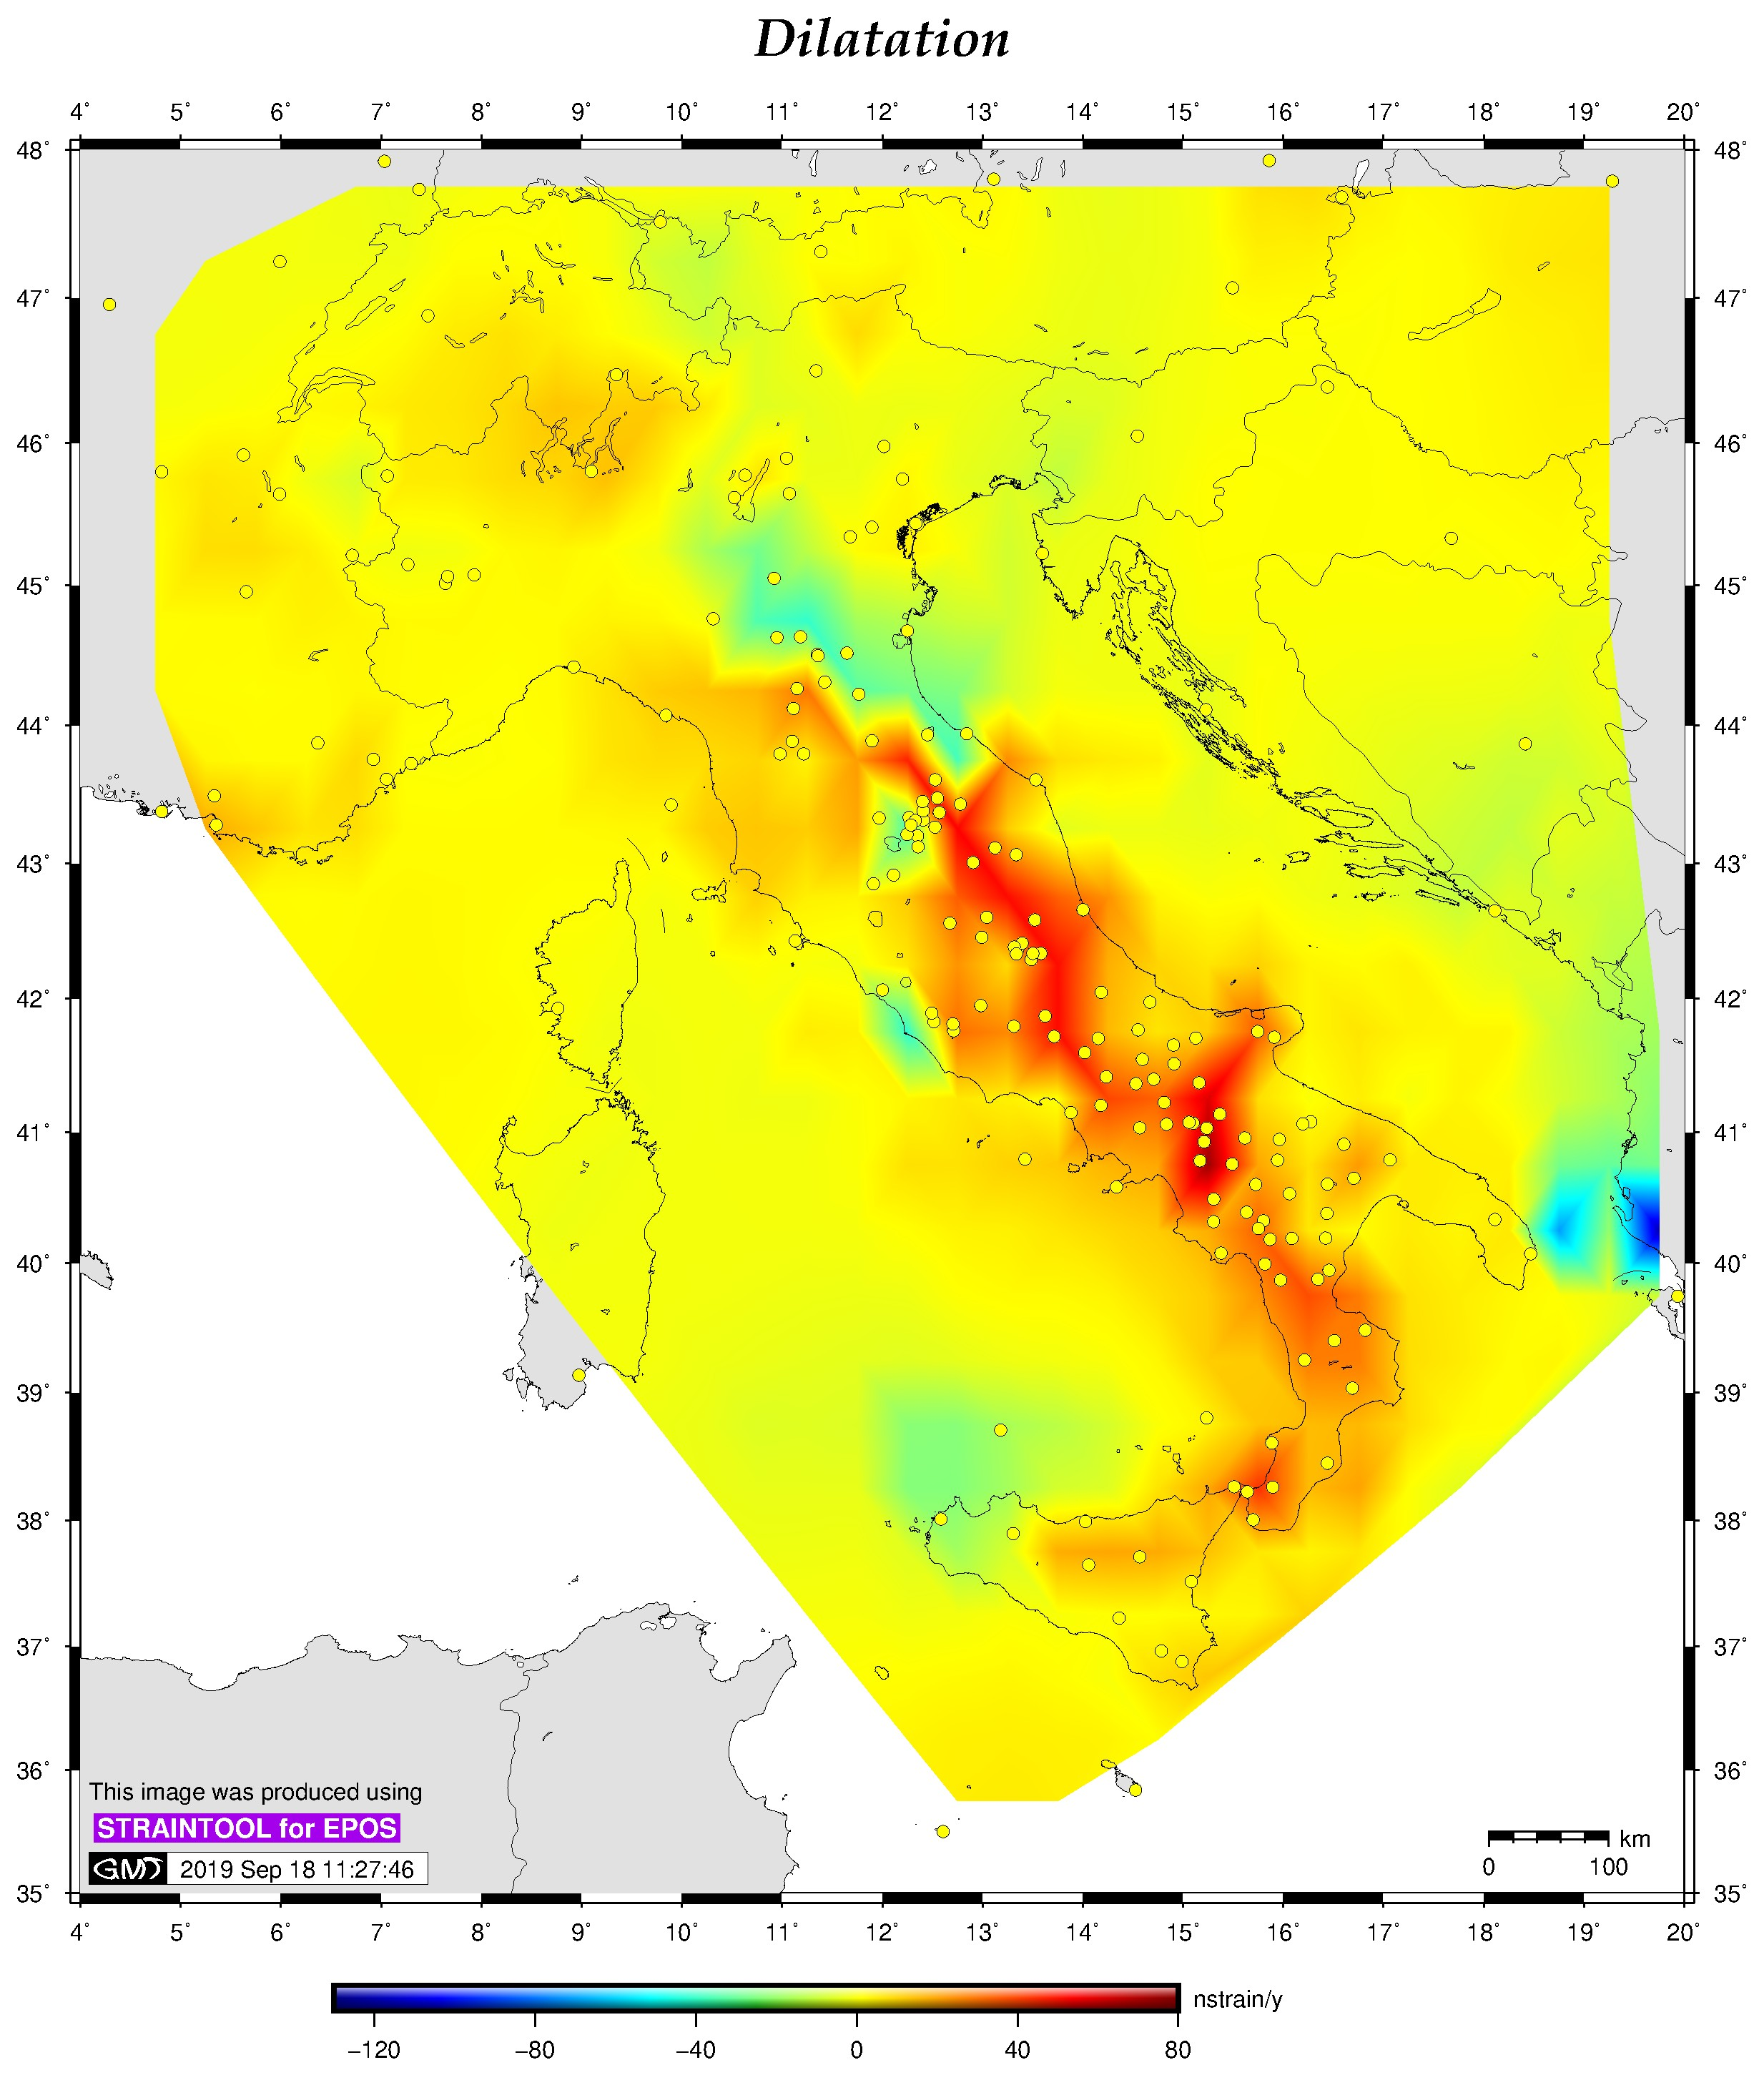
\includegraphics[width=0.9\textwidth]{itmidas-output_dil.jpg}     
    \end{center}
    \end{column}
  
  \end{columns}

\end{frame}
\note{}

\begin{frame}
 \frametitle{Statistics}
 \framesubtitle{Sigma value}
 \label{ch4:}
   
  \begin{columns}
    \begin{column}{0.5\textwidth}
      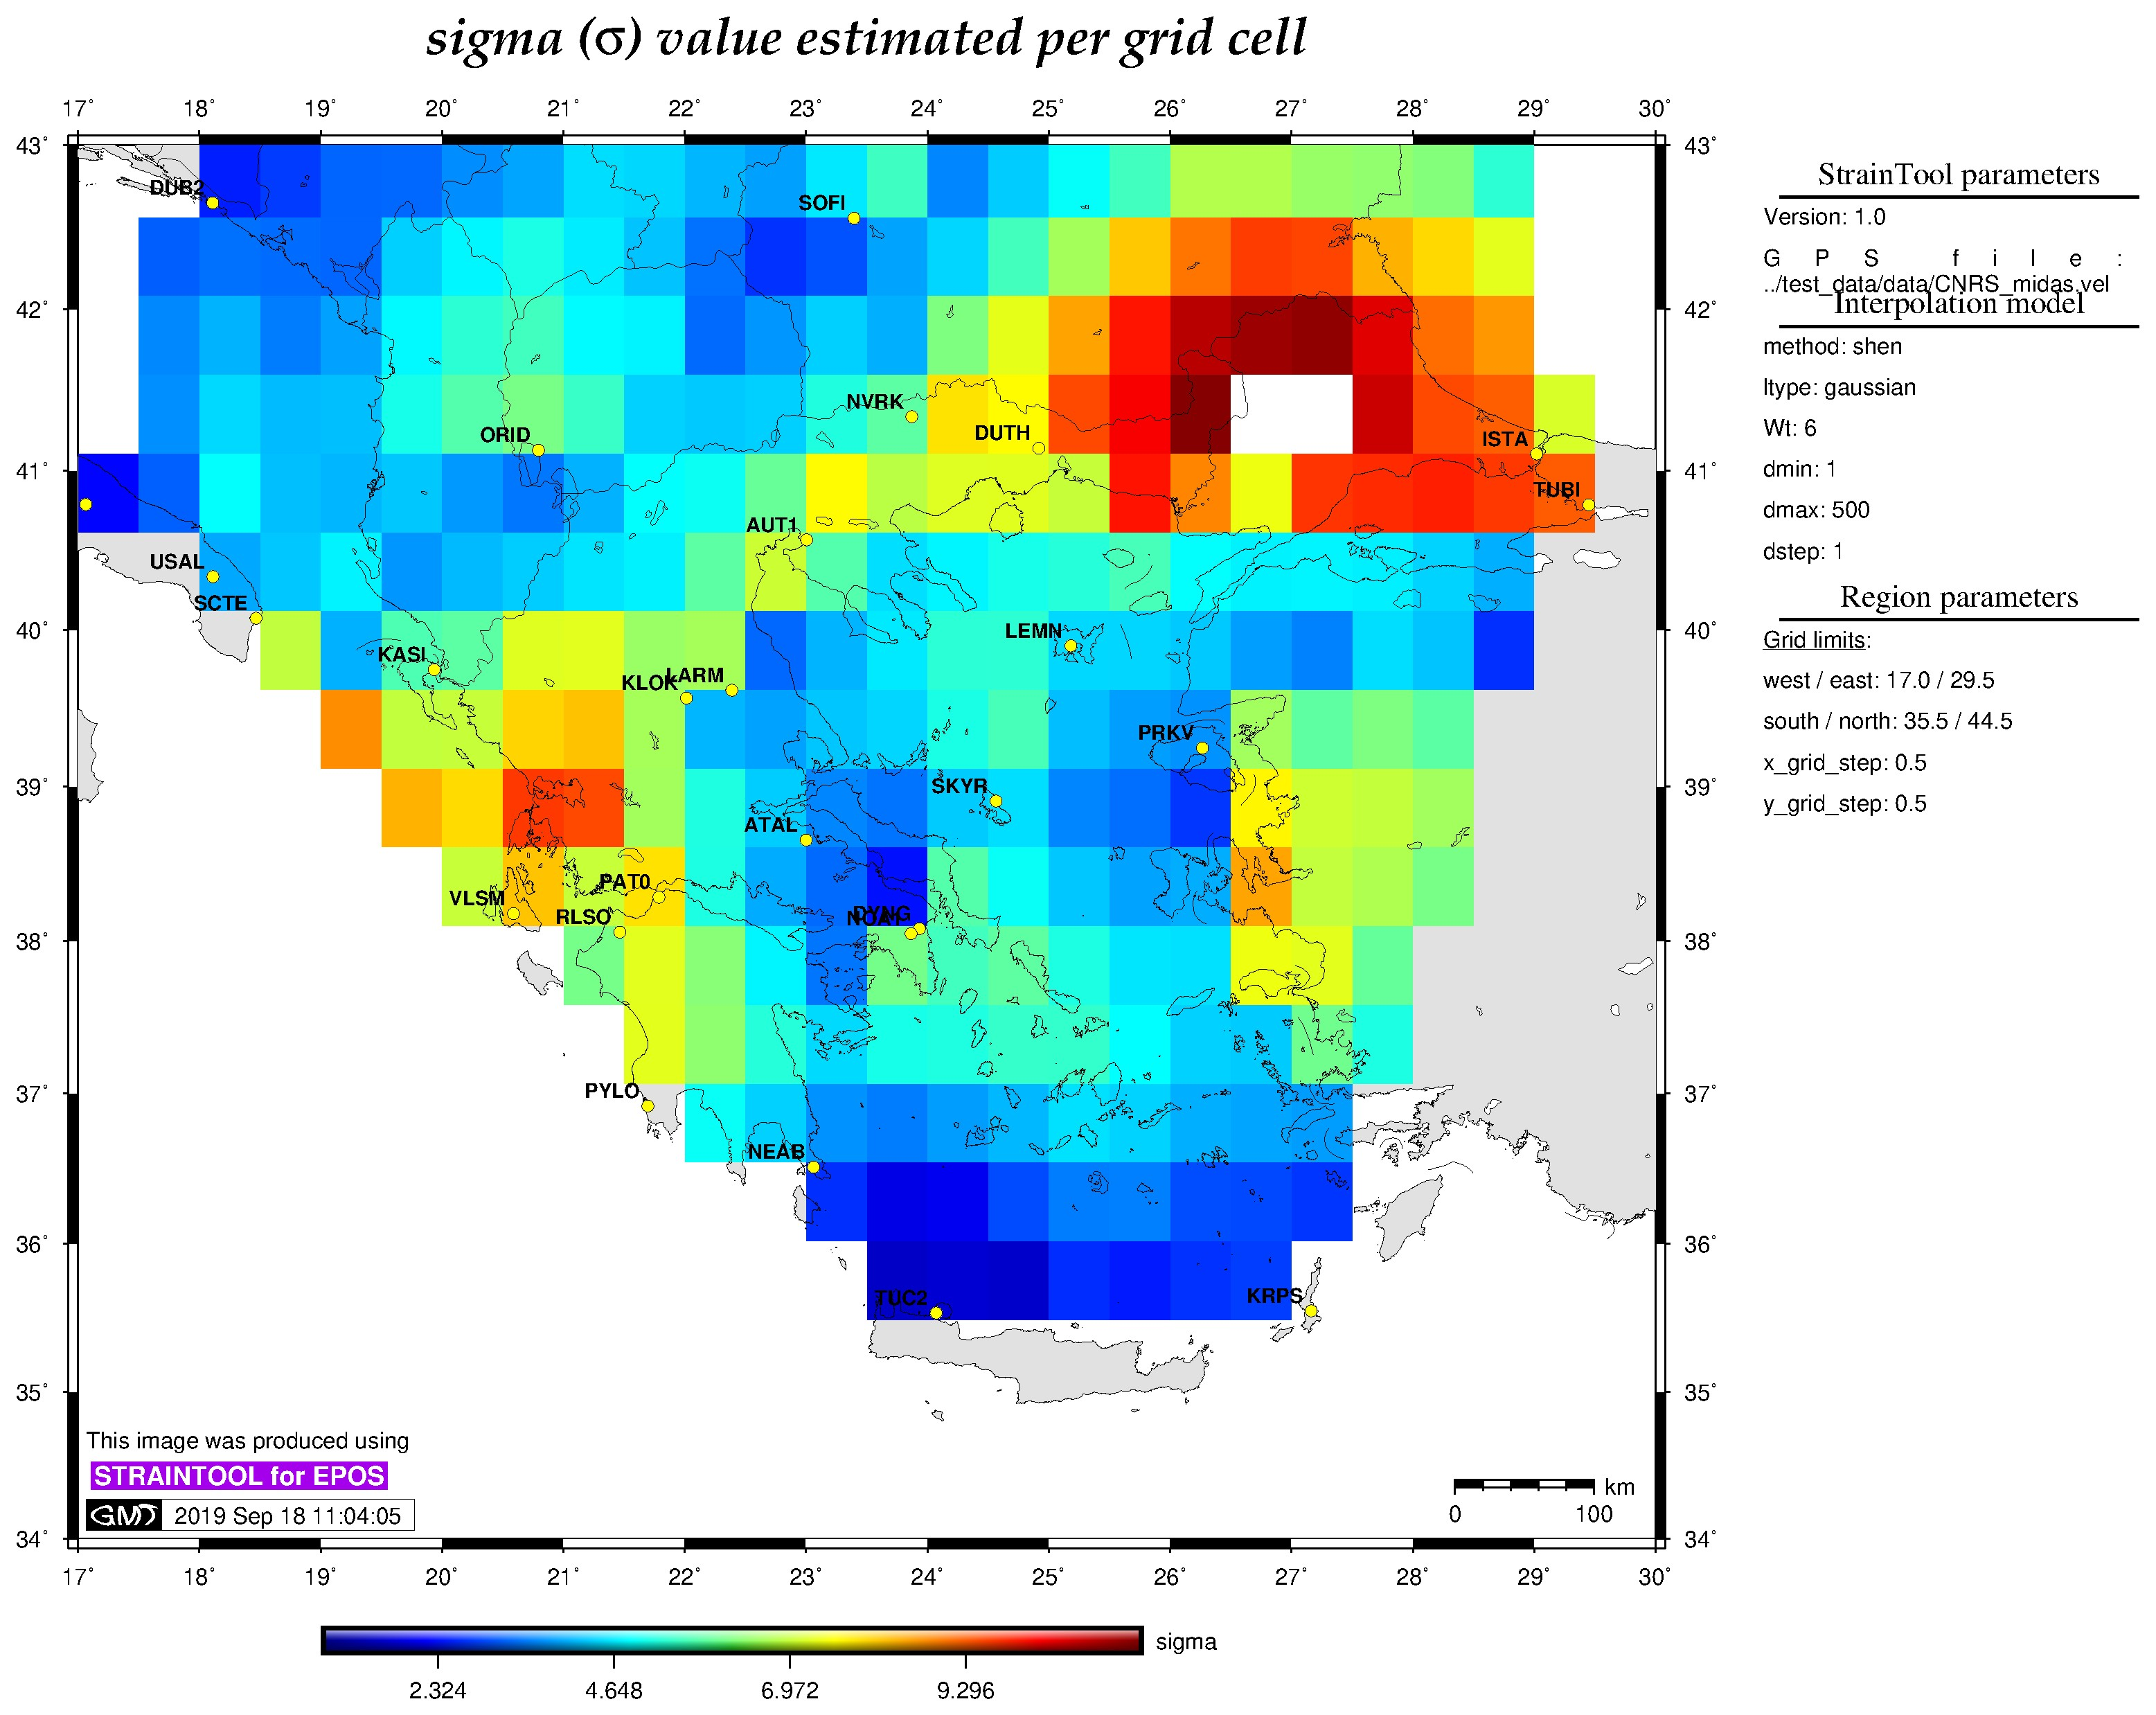
\includegraphics[width=.98\textwidth]{grmidas-output_stats-sigma.jpg}   
    \end{column}
    \begin{column}{0.5\textwidth}
    \begin{center}
      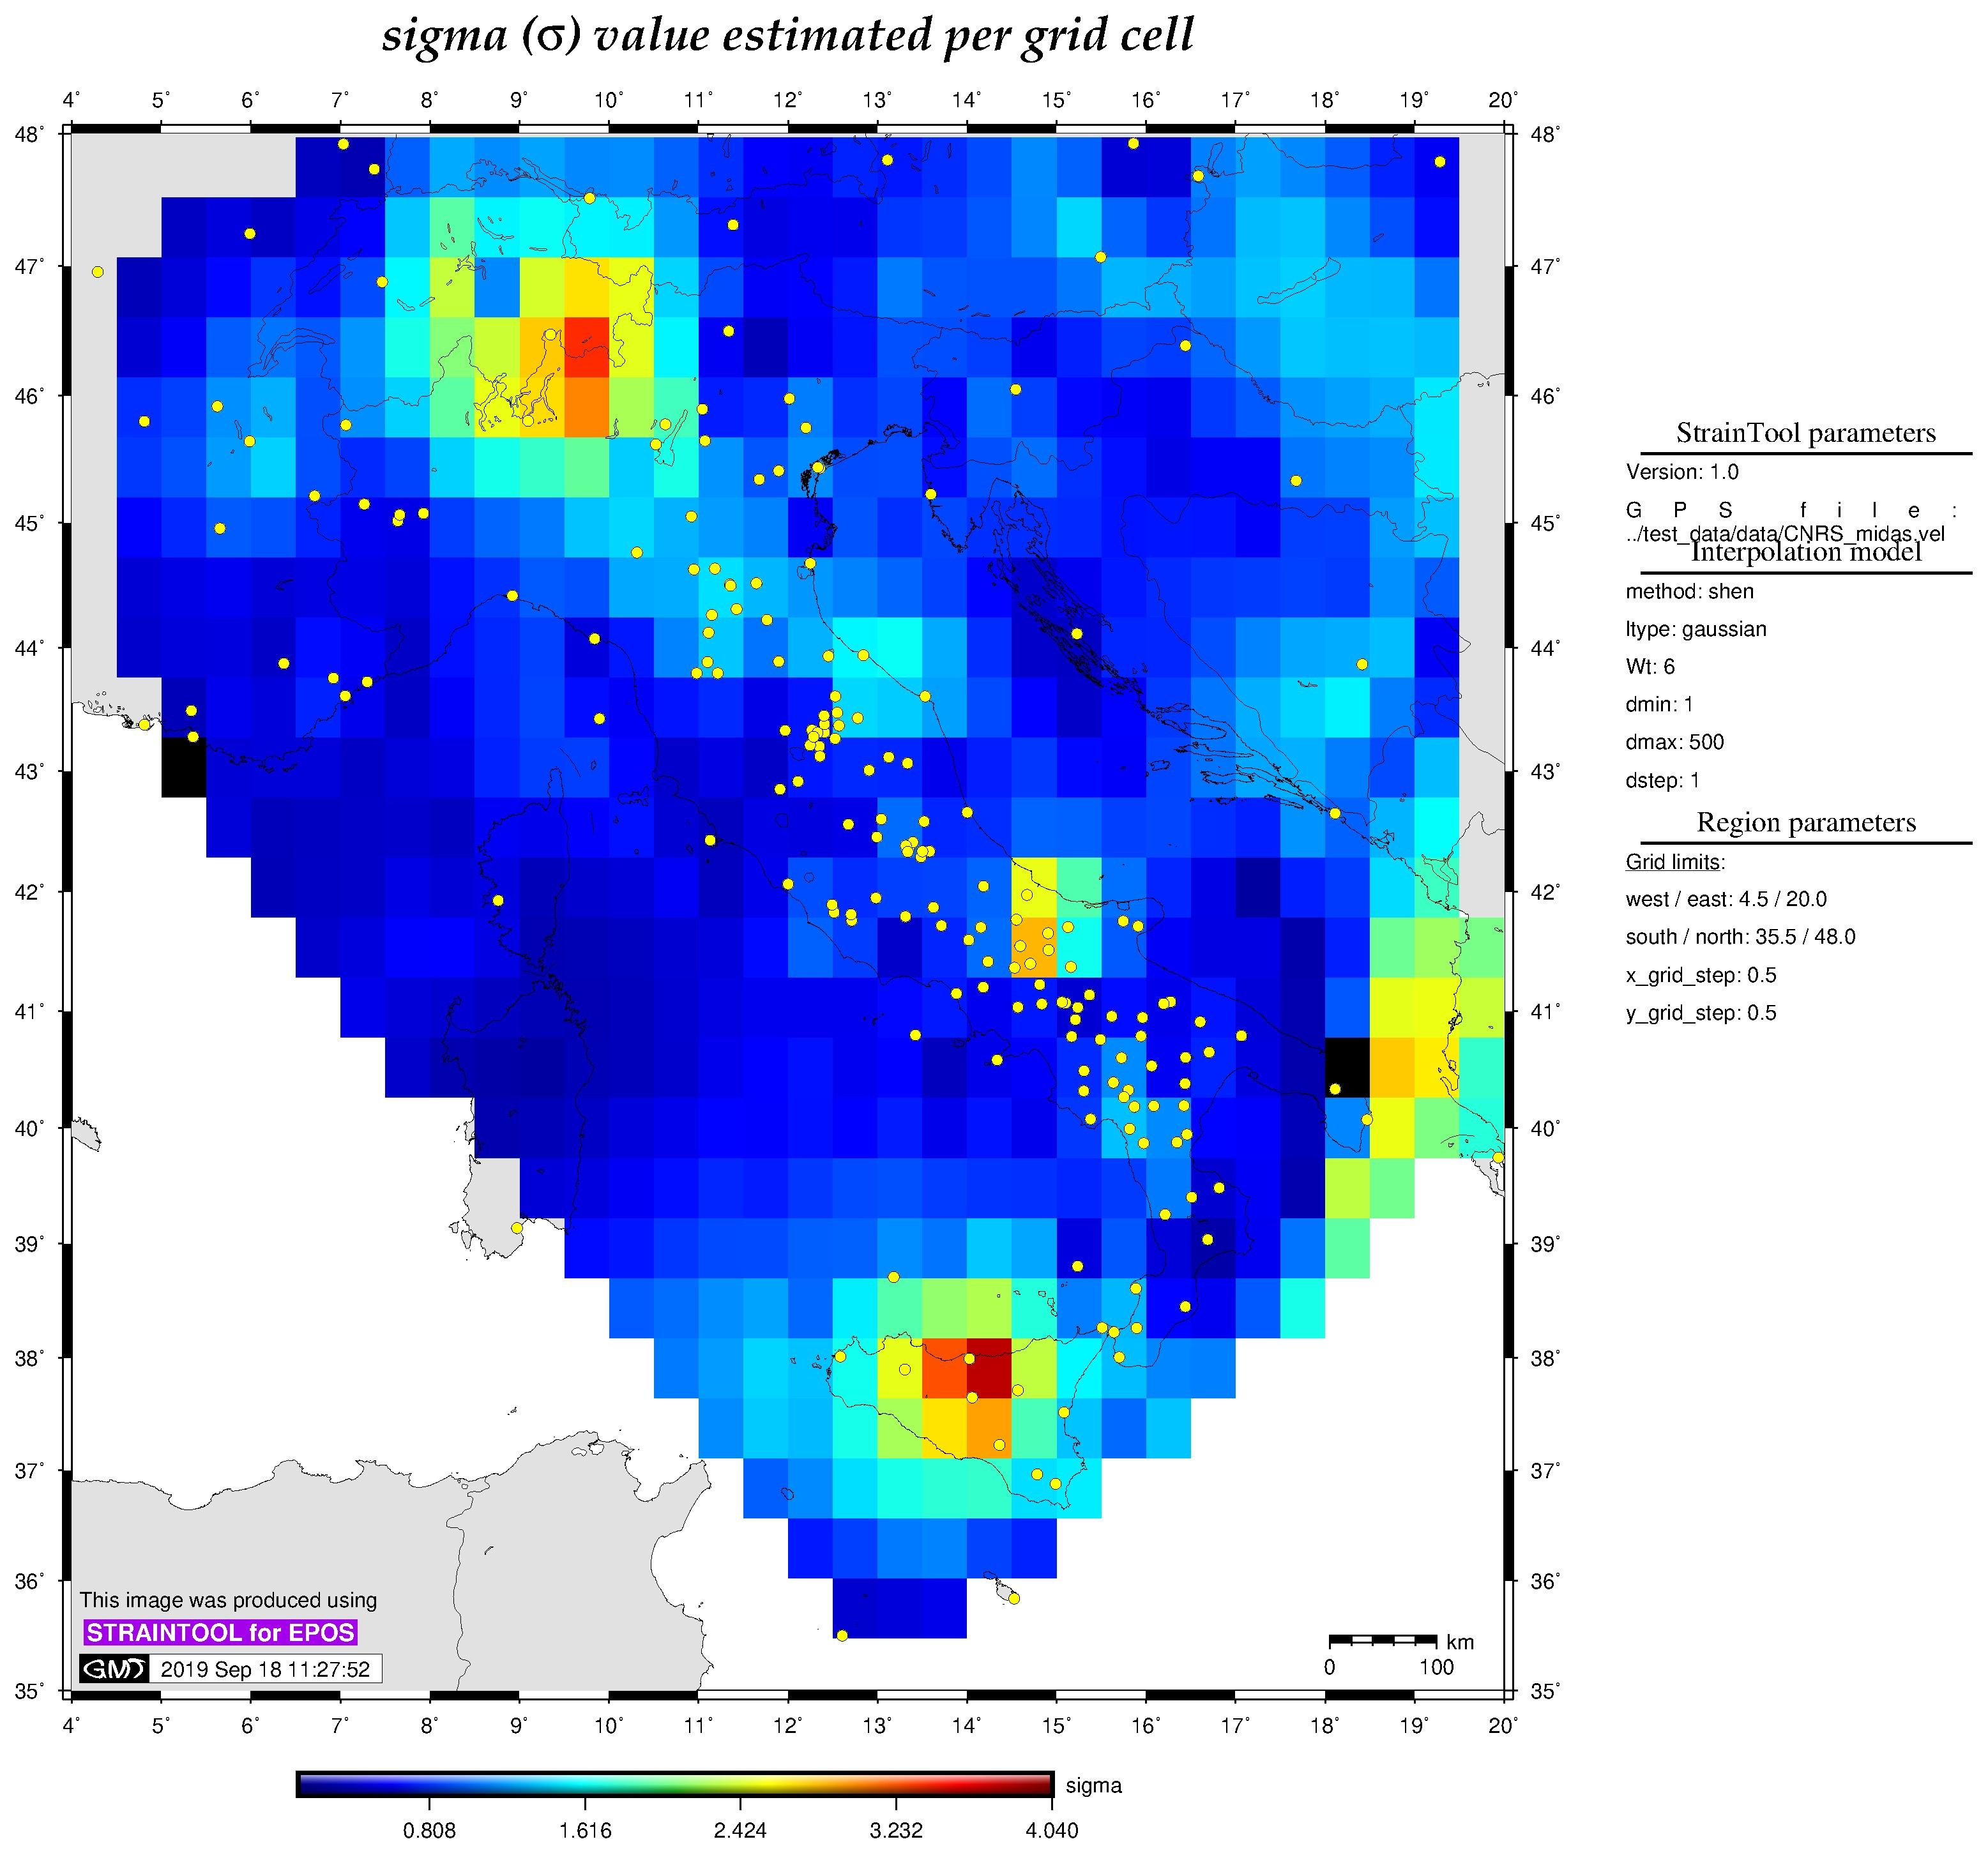
\includegraphics[width=0.98\textwidth]{itmidas-output_stats-sigma.jpg}     
    \end{center}
    \end{column}
  
  \end{columns}

\end{frame}
\note{}

\begin{frame}
 \frametitle{Statistics}
 \framesubtitle{D optimal smoothing parameter}
 \label{ch4:}
   
  \begin{columns}
    \begin{column}{0.5\textwidth}
      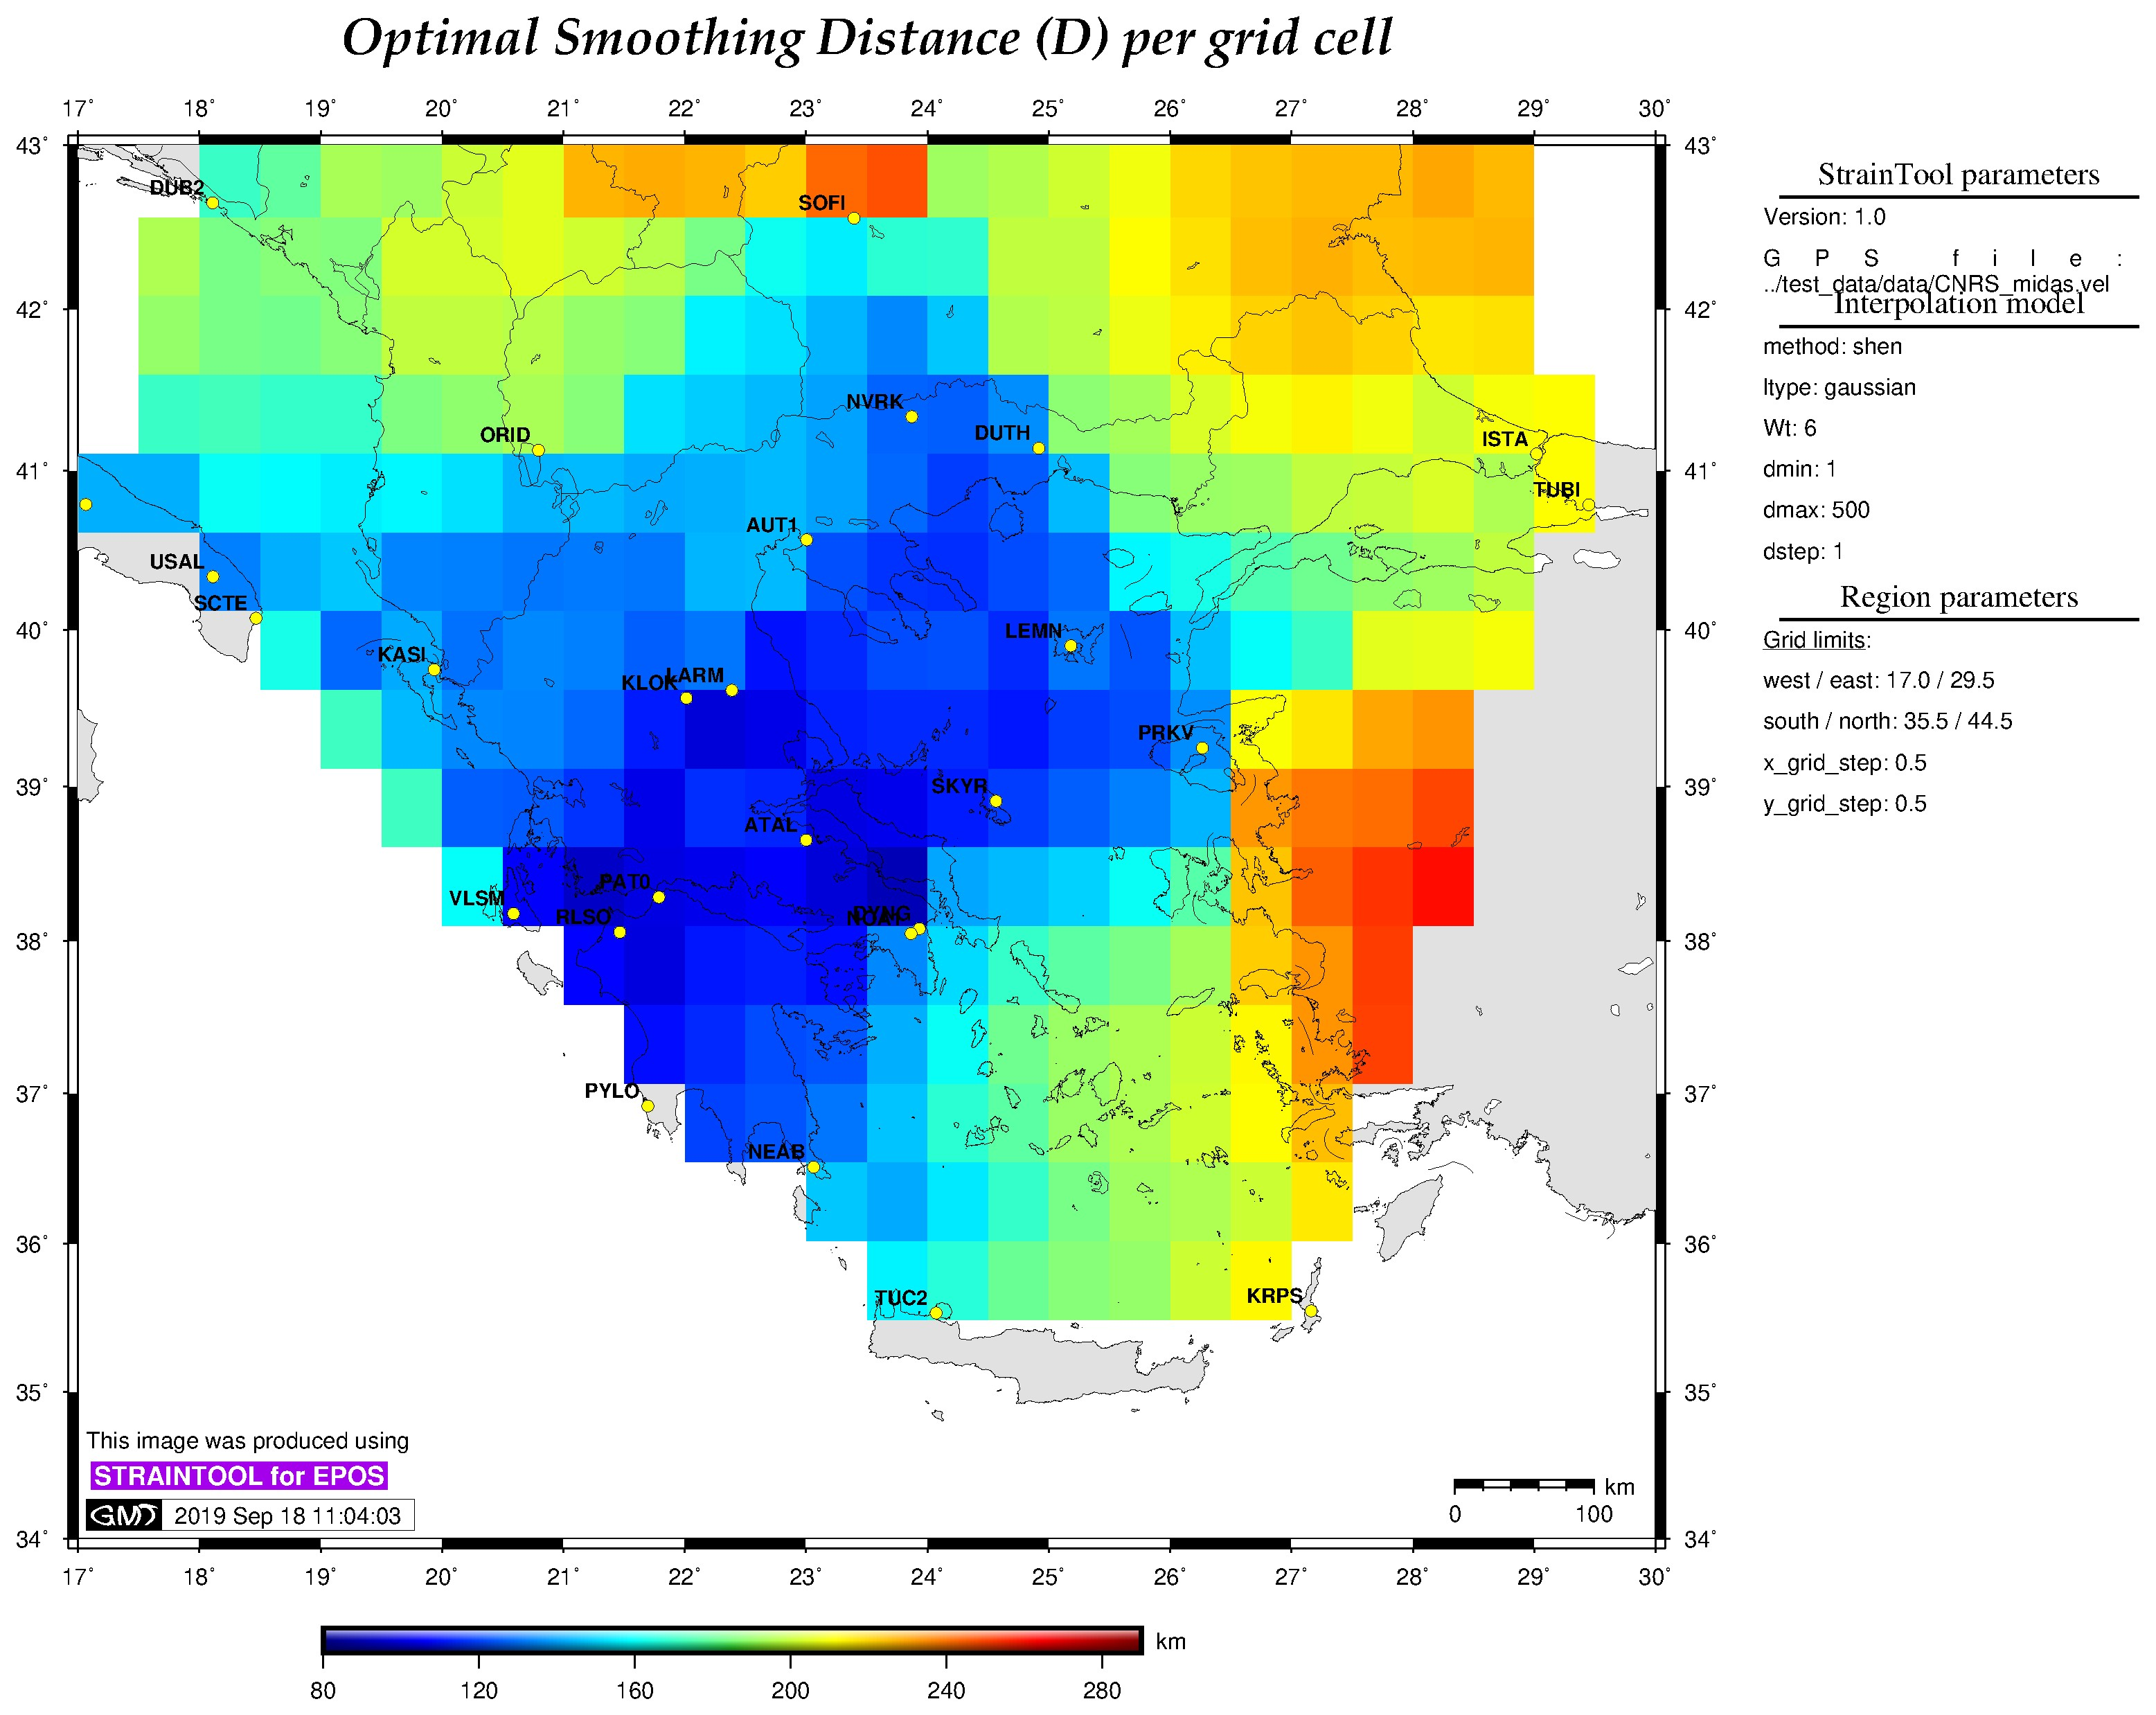
\includegraphics[width=.98\textwidth]{grmidas-output_stats-doptimal.jpg}   
    \end{column}
    \begin{column}{0.5\textwidth}
    \begin{center}
      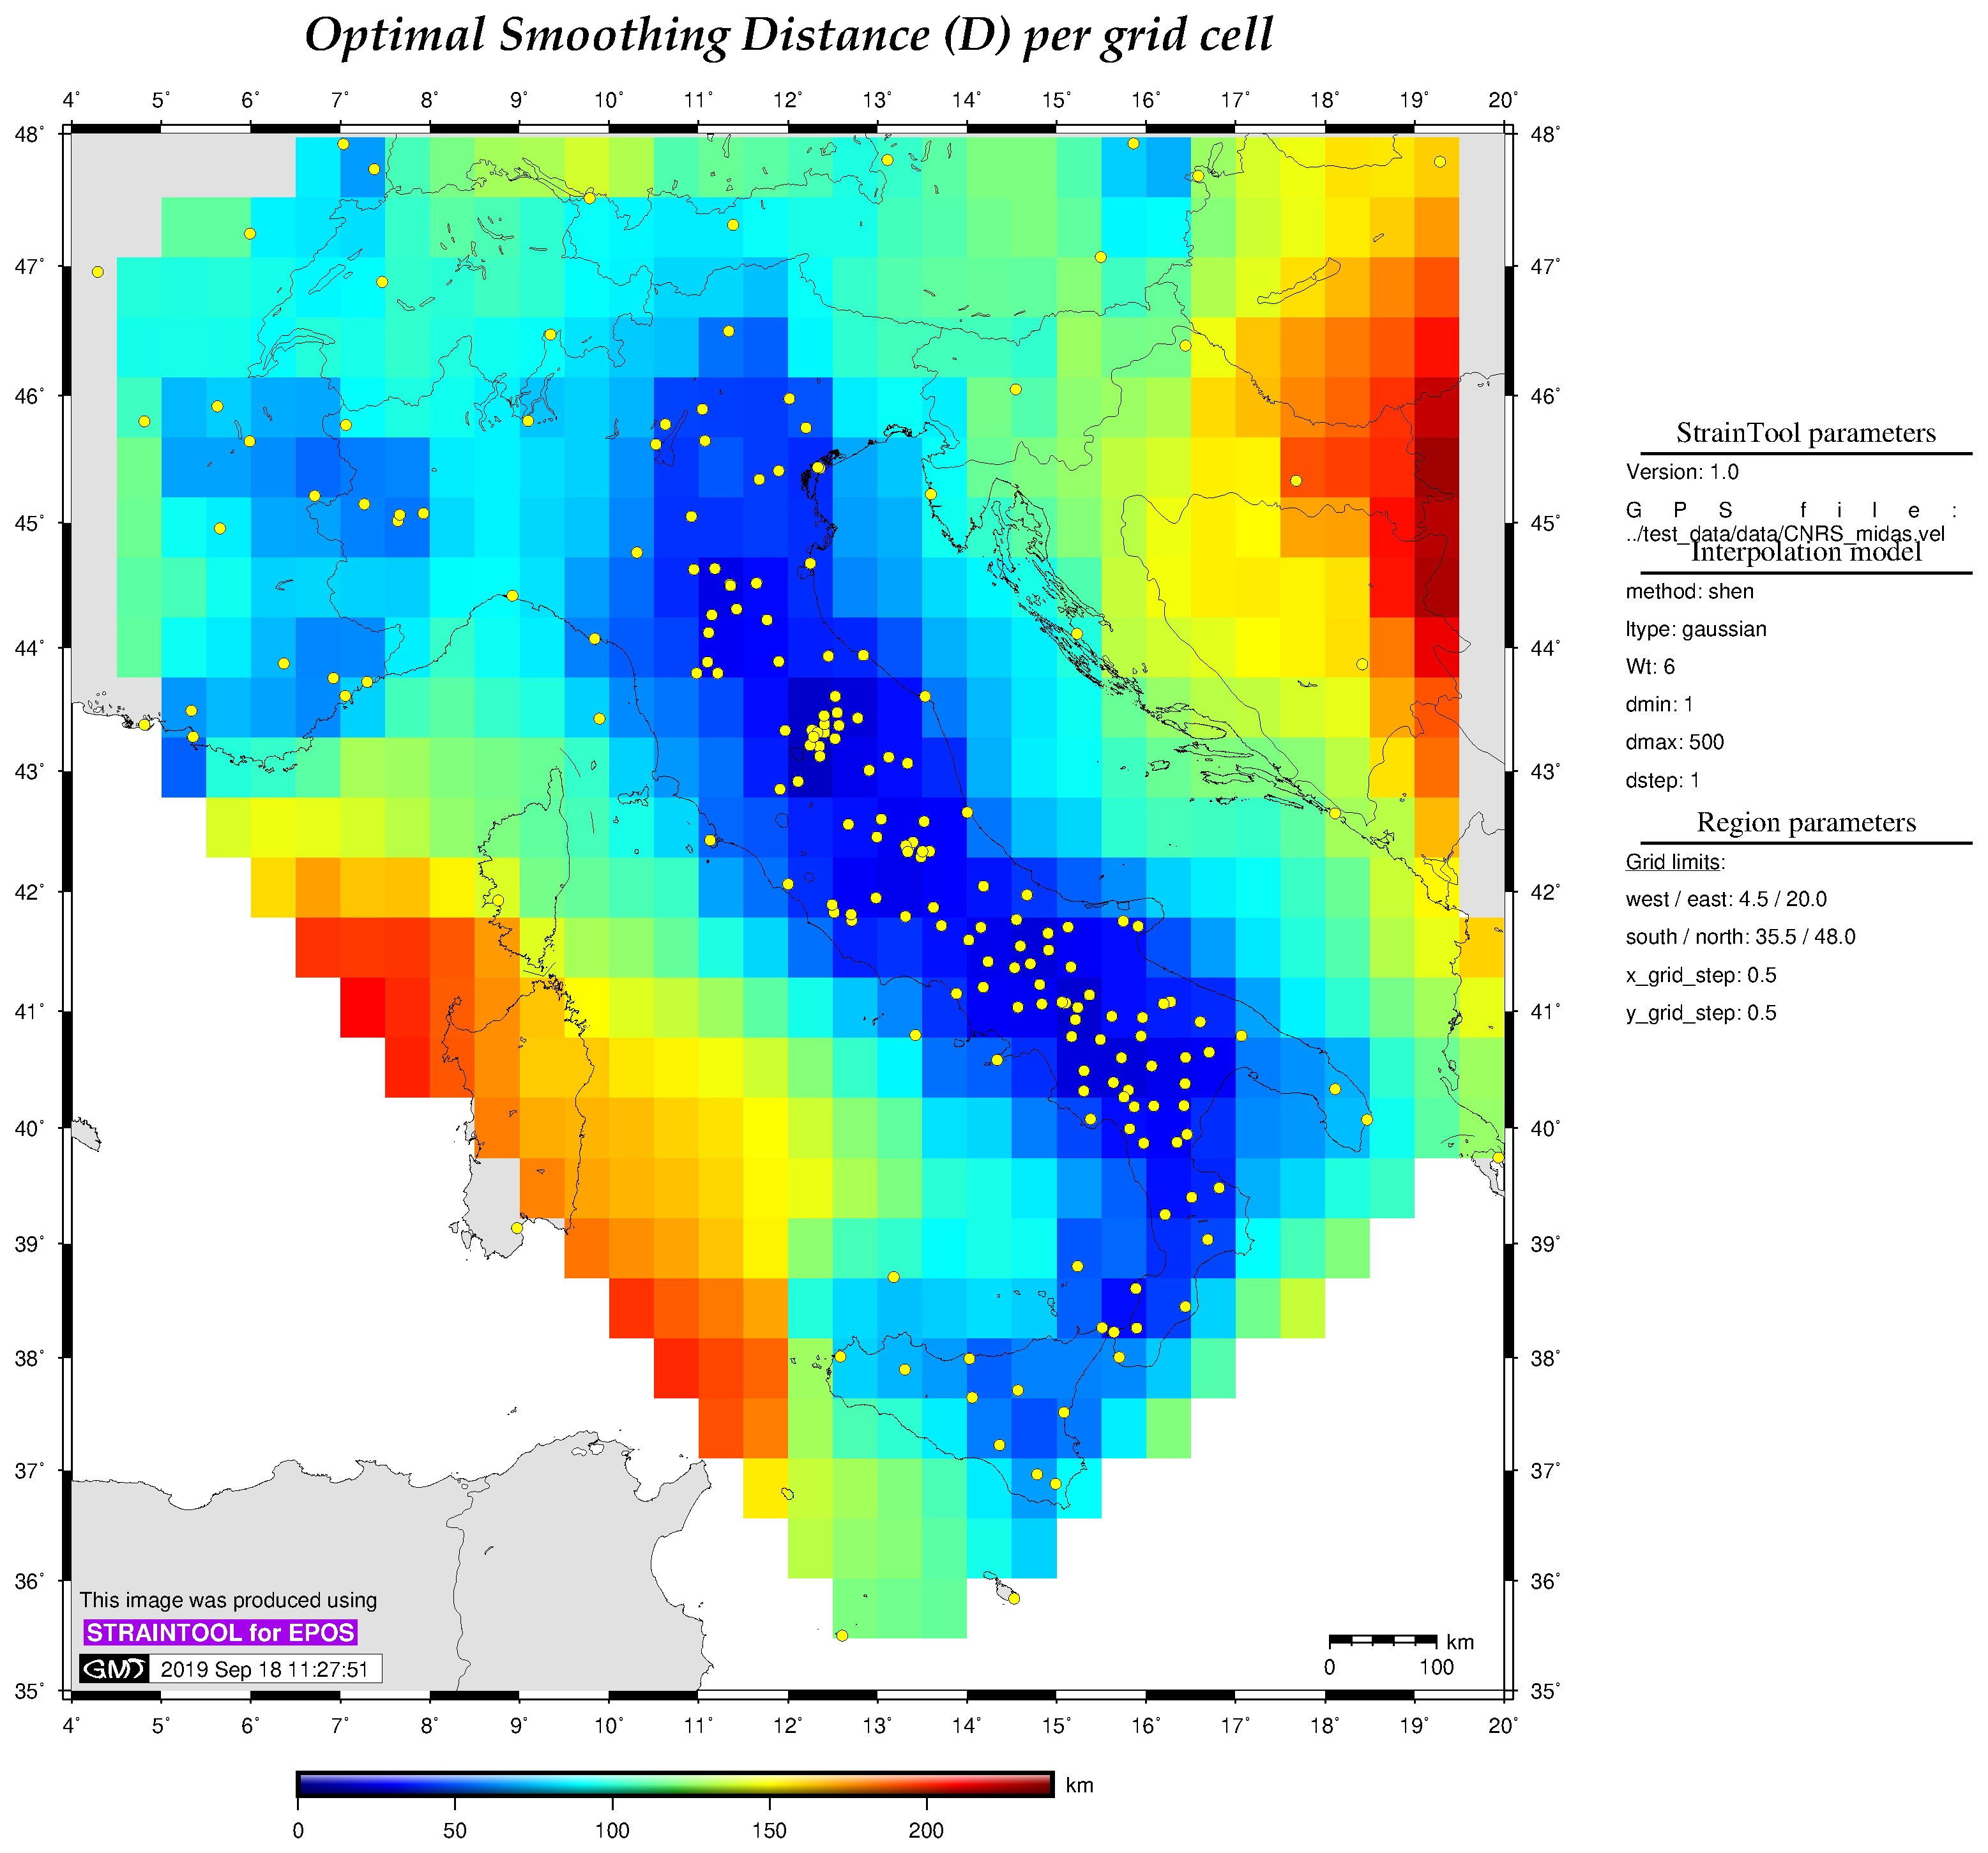
\includegraphics[width=0.98\textwidth]{itmidas-output_stats-doptimal.jpg}     
    \end{center}
    \end{column}
  
  \end{columns}

\end{frame}
\note{}

%\begin{frame}
%  \frametitle{}
%  \framesubtitle{}
%  \label{ch4:}

%\end{frame}
%\note{}
